%% 
%% Copyright 2019-2021 Elsevier Ltd
%% 
%% This file is part of the 'CAS Bundle'.
%% --------------------------------------
%% 
%% It may be distributed under the conditions of the LaTeX Project Public
%% License, either version 1.2 of this license or (at your option) any
%% later version.  The latest version of this license is in
%%    http://www.latex-project.org/lppl.txt
%% and version 1.2 or later is part of all distributions of LaTeX
%% version 1999/12/01 or later.
%% 
%% The list of all files belonging to the 'CAS Bundle' is
%% given in the file `manifest.txt'.
%% 
%% Template article for cas-sc documentclass for 
%% single column output.

\documentclass[a4paper,fleqn]{cas-sc}

% If the frontmatter runs over more than one page
% use the longmktitle option.

%\documentclass[a4paper,fleqn,longmktitle]{cas-sc}

%\usepackage[numbers]{natbib}
%\usepackage[authoryear]{natbib}
\usepackage{xcolor}
\usepackage{epstopdf}

\usepackage[authoryear,longnamesfirst]{natbib}

%%%Author macros
\def\tsc#1{\csdef{#1}{\textsc{\lowercase{#1}}\xspace}}
\tsc{WGM}
\tsc{QE}
%%%

% Uncomment and use as if needed
%\newtheorem{theorem}{Theorem}
%\newtheorem{lemma}[theorem]{Lemma}
%\newdefinition{rmk}{Remark}
%\newproof{pf}{Proof}
%\newproof{pot}{Proof of Theorem \ref{thm}}

\begin{document}
\let\WriteBookmarks\relax
\def\floatpagepagefraction{1}
\def\textpagefraction{.001}

% Short title
\shorttitle{Interface formulation for GFDM for groundwater flow}    

% Short author
\shortauthors{C. Ch\'avez {\em et al}}  

% Main title of the paper
\title [mode = title]{Interface formulation for generalized finite difference method for solving groundwater flow}  

% Title footnote mark
% eg: \tnotemark[1]
%%%\tnotemark[<tnote number>] 

% Title footnote 1.
% eg: \tnotetext[1]{Title footnote text}
%%%\tnotetext[<tnote number>]{<tnote text>} 

% First author
%
% Options: Use if required
% eg: \author[1,3]{Author Name}[type=editor,
%       style=chinese,
%       auid=000,
%       bioid=1,
%       prefix=Sir,
%       orcid=0000-0000-0000-0000,
%       facebook=<facebook id>,
%       twitter=<twitter id>,
%       linkedin=<linkedin id>,
%       gplus=<gplus id>]

\author[1]{C. Ch\'avez-Negrete}[orcid=0000-0002-3932-6943]

% Corresponding author indication
%\cormark[1]

% Footnote of the first author
%%%\fnmark[<footnote mark no>]

% Email id of the first author
\ead{cchavez@umich.mx}

% URL of the first author
%%%\ead[url]{<URL>}

% Credit authorship
% eg: \credit{Conceptualization of this study, Methodology, Software}
%%%\credit{<Credit authorship details>}

% Address/affiliation
\affiliation[1]{organization=Facultad de Ingenier\'ia Civil, U.M.S.N.H.,
            addressline={Edificio C, Ciudad Universtaria}, 
            city={Morelia},
%          citysep={}, % Uncomment if no comma needed between city and postcode
            postcode={58040}, 
            state={Michoac\'an},
            country={M\'exico}}

\author[2]{F.J. Dom\'inguez-Mota}[orcid=0000-0001-6837-172X]

\cormark[1]
% Footnote of the second author
%%%\fnmark[2]

% Email id of the second author
\ead{dmota@umich.mx}

% URL of the second author
%%%\ead[url]{}

% Credit authorship
%%%\credit{}

% Address/affiliation
\affiliation[2]{organization=Facultad de Ciencias F\'isico Matem\'aticas, U.M.S.N.H.,
            addressline={Edificio B, Ciudad Universitaria}, 
            city={Morelia},
%          citysep={}, % Uncomment if no comma needed between city and postcode
            postcode={58040}, 
            state={Michoac\'an},
            country={M\'exico}}

% Corresponding author text
\cortext[1]{Corresponding author}

% Footnote text
%%%\fntext[1]{}

% For a title note without a number/mark
%\nonumnote{}

%%%
\author[2]{R. Rom\'an-Guti\'errez}[orcid=0000-0001-8521-9391]

% Footnote of the second author
%%%\fnmark[2]

% Email id of the second author
\ead{ricardo.roman@umich.mx}

% URL of the second author
%%%\ead[url]{}

% Credit authorship
%%%\credit{}

% Address/affiliation
%%\affiliation[2]{organization=Facultad de Ciencias F\'isico Matem\'aticas, U.M.S.N.H.,
%%            addressline={Edificio B, Ciudad Universitaria}, 
%%            city={Morelia},
%%%          citysep={}, % Uncomment if no comma needed between city and postcode
%%            postcode={58040}, 
%%            state={Michoac\'an},
%%            country={M\'exico}}

% Corresponding author text
%%%\cortext[1]{Corresponding author}

% Footnote text
%%%\fntext[1]{}
%%%
% Here goes the abstract
\begin{abstract}
Simulation of realistic groundwater flow phenomena in unsaturated porous layered media needs to consider all the environmental features that influence the governing equation of the dynamics of the process, namely, the Richards equation. In the stationary case, the latter is a nonlinear parabolic expression whose numerical solution requires an adequate discretization of the differential operator for approximating its solution accurately to avoid numerical inaccuracies that yield unrealistic numerical oscillations between soil layers. A reliable spatial discretization can be obtained via a generalized finite differences scheme used as a meshless method, which allows the pose of discrete expressions for differential operators, including the discontinuous coefficients that describe the changes in permeability in different media. The key idea is to use a frontier nodal balance expression written so that the amount of water is conserved at the interface nodes. The proposed discretization's robustness and accuracy are demonstrated by presenting several benchmark problems.  
\end{abstract}

% Use if graphical abstract is present
%\begin{graphicalabstract}
%\includegraphics{}
%\end{graphicalabstract}

% Research highlights
%%%\begin{highlights}
%%%\item 
%%%\item 
%%%\item 
%%%\end{highlights}

% Keywords
% Each keyword is seperated by \sep
\begin{keywords}
Layered materials \sep Generalized finite differences \sep  Interface balance \sep Richards equation \sep Discontinuous coefficients 
\end{keywords}

\maketitle

% Main text
\section{Introduction}

The numerical modeling of real-world water flow phenomena in unsaturated porous media must take into account all environmental factors that affect the governing equation of the process dynamics, namely, the Richards equation (1931). The latter degenerates from an elliptic nonlinear expression to a nonlinear parabolic one in the stationary case; in both cases, a thorough numerical procedure is required to get an accurate approximation. One of the features that makes Richards equation hard to solve appears when the domain is a layered medium characterized by discontinuous permeability values. Solving the equation with discontinuous coefficients is a challenging numerical problem encountered frequently in various application fields, particularly in hydrology and soil science. This form of the Richards equation is crucial for understanding groundwater movement in many areas, such as geotechnical engineering and environmental applications.

The finite element method (FEM) is a standard numerical method that has been used to solve Richards equation (\cite{chen2008numerical}, \cite{fredlund2012}, \cite{venkatesh2016distribution}, \cite{luo2021isoparametric}), and it is widely used in geotechnical engineering practice to solve groundwater flow problems (\cite{galavi2010groundwater},\cite{desai2013advanced}, \cite{geo2022heat}). The Finite Volume Method (FVM) is less used than the FEM, but since it is a conservative, it becomes an attractive alternative (\cite{pour2011numerical},\cite{caviedes2013verification}, and \cite{deng2017saturated}). However, in the case of discontinuities, any numerical method must be meticulously configured to effectively capture and deliver precise solutions. Numerous authors with different numerical techniques have explored the solution of equations with discontinuous coefficients; two of the most successful are the Discontinuous Galerkin Method, an adaptation of FEM, and the FVM. When finite elements are defined, the key feature is that the basis functions used for approximation are discontinuous at element boundaries. This discontinuity allows for more flexibility in capturing solutions with discontinuities or shocks using stabilization techniques (\cite{arnold2000discontinuous}, \cite{brezzi2005mixed}, \cite{arnold2005family}, \cite{cockburn2012discontinuous}). This is combined with a feature that is characteristic of the finite volume method, the use of numerical fluxes to account for the discontinuities between neighboring elements; numerical fluxes are introduced at the element interfaces (\cite{ewing2001modified},\cite{boyer2008finite}). These fluxes ensure the conservation of physical quantities and continuity across element boundaries.

On the other hand, the classical Finite Difference (FD) method has also been used extensively to solve the water flow problem in unsaturated layered soil in one dimension (\cite{romano1998numerical},\cite{szymkiewicz2011comparison} and \cite{zhu2020improved}).{ A reliable spatial discretization of the differential operator can be obtained via a Generalized Finite Differences Method (GFDM) in two and three dimensions, making GFDM a powerful technique to solve differential equations using irregular grids of points (\cite{tiwari2003finite},\cite{benito2003h},\cite{benito2001influence},\cite{benito2007solving}). This method is handy for solving engineering problems in homogenous media (\cite{Urena2011appli,chavez2018numerical,tinoco2018stability,li2019generalized,tinoco2020study,zhang2020solving,chavez2021,roman2022numerical}). More recently, the GFDM has been used to solve problems in multi-layered elastic materials (\cite{wang2018domain}, \cite{wang2020domain}) using a non-overlapping decomposition. In each sub-domain, the solution is approximated by the GFDM scheme. At the interface nodes, where the coefficients are discontinuous, it is required to use piecewise constant approximations for the coefficients, matching the values on both sides of the discontinuity. The compatibility of displacements and equilibrium of stresses are imposed on the interface. However, more research using GFDM applied to layered domains is still needed since finite difference coefficients can encounter challenges in accurately capturing the discontinuities when dealing with discontinuous coefficients, leading to numerical oscillations and instability. Special treatments which resemble flux functions may be required to handle discontinuities effectively. This work presents a new technique for approximating water flow in layered soils using the GFDM.}

The proposed technique uses a water balance condition at the interface nodes between two medium layers, a formulation that can be intuitively extended to a $n$-layer interface. As a validation of the proposed method, the results are compared to those of the same problem using the FEM due to the lack of an exact solution. In the first part of the validation, fundamental stationary problems are solved to test the solution on the interface. Afterward, classic water flow problems in dams are solved, considering saturated and unsaturated soils using the same mesh of points in both methods.

\section{Generalized finite difference method formulation}\label{gfdm}

The second-order linear operator, $L$, applied to the hydraulic total head $h$, yields the equation (\ref{eq1})

\begin{equation}
  Lh=A\frac{\partial ^2 h}{\partial x^2}+B\frac{\partial ^2 h}{\partial \text{xy}}+C\frac{\partial ^2 h}{\partial y^2}+D\frac{\partial h}{\partial x}+E\frac{\partial h}{\partial y}+F h . 
  \label{eq1}
\end{equation}

{ 

Let $p_0, p_1, ...,p_q$ be coordinate points in the domain of $Lh$ (Figure \ref{fig0}). The generalized finite difference method is based on providing an approximation $L_0 h$ to  $Lh$ from the first terms of its Taylor series, which expresses $h(p_0)$ as a linear combination of values $h(p_1)$ to $h(p_q)$ of the variable $h$ (water total head, in this case), namely,

\begin{equation}\label{eq2}
L_0 h=\underset{i=0}{\overset{q}{\Sigma }}\Gamma _i h(p_i),
\end{equation}

where $\Gamma_i$ are weights values that need to be set to achieve consistency, {\em id est}, it is required that the local truncation error $\tau$ approaches zero as the points $p_1, ...,p_q$ tend to $p_0$, which yields

\begin{equation}
\tau= Lh- L_0 h=A\frac{\partial ^2 h}{\partial x^2}+B\frac{\partial ^2 h}{\partial \text{xy}}+C\frac{\partial ^2 h}{\partial y^2}+D\frac{\partial h}{\partial x}+E\frac{\partial h}{\partial y}+F h -
\underset{i=0}{\overset{q}{\Sigma }}\Gamma _i h(p_i)\to \text{0}
\label{eq3}
\end{equation}

}

\begin{figure}[htb]
  \centering
  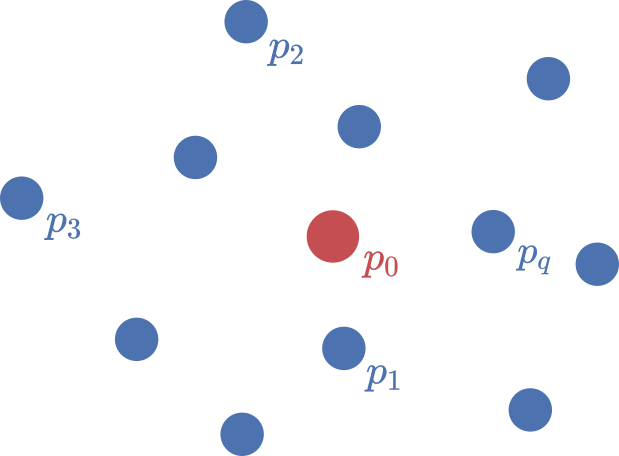
\includegraphics[width=.3\linewidth]{points.png}
  \caption{Points $p_0,\cdots,p_q$}
  \label{fig0}
\end{figure}  

Considering the Taylor series of $\tau$ up to the second order and reordering the resulting expression, the linear system (\ref{eq4}) can be posed:

\begin{equation}
  \left(
    \begin{array}{rrrrr}
    1&  &1 &... & 1\\
    0&  &\Delta x_1 &... &\Delta x_q\\
    0&  &\Delta y_1 &... &\Delta y_q\\
    0&  &(\Delta x_1)^2 &... &(\Delta x_q)^2\\
    0&  &\Delta x_1\Delta y_1 &... &\Delta x_q\Delta y_q\\
    0&  &(\Delta y_1)^2 &... &(\Delta y_q)^2\\
    \end{array}
    \right)
    \left(
    \begin{array}{lclcl}
    \Gamma_0\\
    \Gamma_1\\
    \Gamma_2\\
    .\\
    .\\
    .\\
    \Gamma_q\\
    \end{array}
    \right)=
    \left(
    \begin{array}{rclcl}
    F(x_0,y_0)\\
    D(x_0,y_0)\\
    E(x_0,y_0)\\
    2A(x_0,y_0)\\
    B(x_0,y_0)\\
    2C(x_0,y_0)\\
    \end{array}
    \right) . 
    \label{eq4}
\end{equation}

{
It must be noted that, if required, the adaptable choice of Taylor series expansions can be used to define varying-order expansions. More neighbors can be used if the aim is to pose a higher-order method. But more order implies more computational costs, and certainly some problems -like those with very high gradient norms- might require higher-order methods, but equation (\ref{eq4}) is aimed at providing a straightforward extension of the classical second-order schemes on rectangular grids, because such accuracy is used in a large number of applications.
}

System (\ref{eq4}) is a block matrix one. Splitting the first equation of the system (\ref{eq4})

\begin{equation}\label{eq5}
  \sum _{i=1}^q \Gamma_i=F(x_0,y_0),
\end{equation}

the system is simplified as

\begin{equation}\label{eq6}
\left(
\begin{array}{clcl}
\Delta x_1 &... &\Delta x_q\\
\Delta y_1 &... &\Delta y_q\\
(\Delta x_1)^2 &... &(\Delta x_q)^2\\
\Delta x_1\Delta y_1 &... &\Delta x_q\Delta y_q\\
(\Delta y_1)^2 &... &(\Delta y_q)^2\\
\end{array}
\right)
\left(
\begin{array}{lclcl}
\Gamma_1\\
\Gamma_2\\
.\\
.\\
.\\
\Gamma_q\\
\end{array}
\right)=
\left(
\begin{array}{rclcl}
D(x_0,y_0)\\
E(x_0,y_0)\\
2A(x_0,y_0)\\
B(x_0,y_0)\\
2C(x_0,y_0)\\
\end{array}
\right)
\end{equation}

The solution of the equation (\ref{eq6}) can be used to approximate the differential operator (\ref{eq2}) at each point $p_0$. Succinctly, it can be written as

\begin{equation}\label{eq7}
M \Gamma= \beta
\end{equation}

where $\beta$ is a vector of the known values of the coefficients of the differential equation to be solved. It must be noticed that the number of columns of $M$ depends on $q$, the number of neighbor nodes of $p_0$, and, in general, it is not a square matrix.
{
The adequate selection of nodes is essential for getting an accurate approximation to the derivatives and has an important effect, especially on the stability of the time-dependent problems. The seminal paper of Perrone and Kao suggested selecting a node for each octant in a system of Cartesian axes around $p_0$ (\cite{perrone1975general}). Liska presented a thorough analysis of the suitable selection of nodes for several elliptic, parabolic, biharmonic, and nonlinear problems and proposed the so-called four quadrant criterion, which consists of the selection of the two nearest nodes per quadrant (\cite{liszka1980finite}). Benito {\em et al} have studied the effect of the spatial distribution of the nodes in the generalized finite difference method for the classical parabolic equation using a weighted least squares version of the method on rectangular and L-shaped regions (\cite{benito2001influence}). In (\cite{tinoco2018stability,tinoco2020study,roman2022numerical}), the authors addressed the unweighted version of the method and shown several stability results for advection-diffusion problems on very irregular regions without needing the selection of a weight function, which is a remarkable fact, since the use of weight functions requires choosing a suitable function and calibrating its parameters; on the other hand, the unweighted version of the finite differences relies only the accurate solution of system (\ref{eq6}).\\
In the present paper, having in mind that a self-adjoint elliptic operator mainly gives the ansatz, which is even discretized in classical differences as a symmetric matrix operator as a consequence of the self-adjointness, it can be expected that the stencils in the generalized differences given by the spatial distribution of the points $p_0$ to $p_q$ should reflect such symmetry in terms of the distribution of the points around $p_0$. Thus, the grids used in the paper were generated following a Delaunay-like structure, which tends to generate many equilateral triangles in meshes where the average number of neighbors is 6, all located in a very regular structure, and therefore produce full row-rank matrices $M$.
}
If the system (\ref{eq6}) has full row rank, the pseudo-inverse of $M$ can be used to obtain a set of values of $\Gamma$. It is also important to note that in this case, if $p>5$, the kernel of (\ref{eq6}) is nontrivial, and therefore, there is a linear manifold associated with the solutions, or, in other words, there are many possible solutions to choose from.

The remaining value of $\Gamma_0$, is obtained from equation (\ref{eq5})

\begin{equation}
\Gamma _0=F-\underset{i=1}{\overset{q}{\Sigma }}\Gamma _i.
\end{equation}

Given the coefficients $\Gamma$ at each node of the mesh where required, and considering the mesh node connections, the matrix $H$ of coefficients is assembled, and the  discrete system which approximates (\ref{eq1}) can be solved (equation \ref{eq9}) to obtain the values of the head $h$ at the grid nodes: 

\begin{equation}\label{eq9}
H h+f=0,
\end{equation}


here, $f$ is the vector of known values of $h$ at the boundary given by the Dirichlet boundary condition.

\section{Balance at the boundary nodes}\label{sec3}

The balance at each frontier node is formulated as a flow boundary condition (\cite{desai2013advanced}). Intuitively, the flow condition for making the balance is that the sum of the water amount leaving one side of the interface equals the amount of water entering the other side of the interface, naturally, considering the corresponding sign convention. It can be written as    
 
\begin{equation}
\sum_{i=1}^{nl} k_{x_i} \frac{\partial h}{\partial x} l_{x_i}+
\sum_{i=1}^{nl} k_{y_i} \frac{\partial h}{\partial y} l_{y_i}=0,
\label{eq10}
\end{equation}

in cartesian coordinates, where $nl$ is the number of layers, $k_{x_i}$ and $k_{y_i}$ are the permeability values in the directions of $x$ and $y$ respectively, $h$ is the hydraulic total head, and $l_x$ and $l_y$ are the direction cosines of the outward normal to the boundary.  

Figure (\ref{fig1}) presents a sketch of the scheme of nodes on a layered medium; each material is shown separately for the sake of clarity, and, on both sides, there is the $p_0$ node linked to the neighboring nodes on each layer. The node configuration on each side is used to approximate the amount of water flow by the generalized finite differences method on that side. Figure (\ref{fig1}) also indicates the direction of the outward normal to the boundary and the cartesian components of the flow rate $q_{xi}$ and $q_{yi}$; the balance in the $x$ direction will be $ q_{x1}+q_{x2}=0$. Figure \ref{fig2} shows the balance of a point $p_0$ located on a boundary point between three layers. Again, the layers are separated for simplicity, and, for instance, the balance in the $x$ direction is given by $ q_{x1}+ q_{x2}+ q_{x3}=0$.

\begin{figure}[htb]
  \centering
  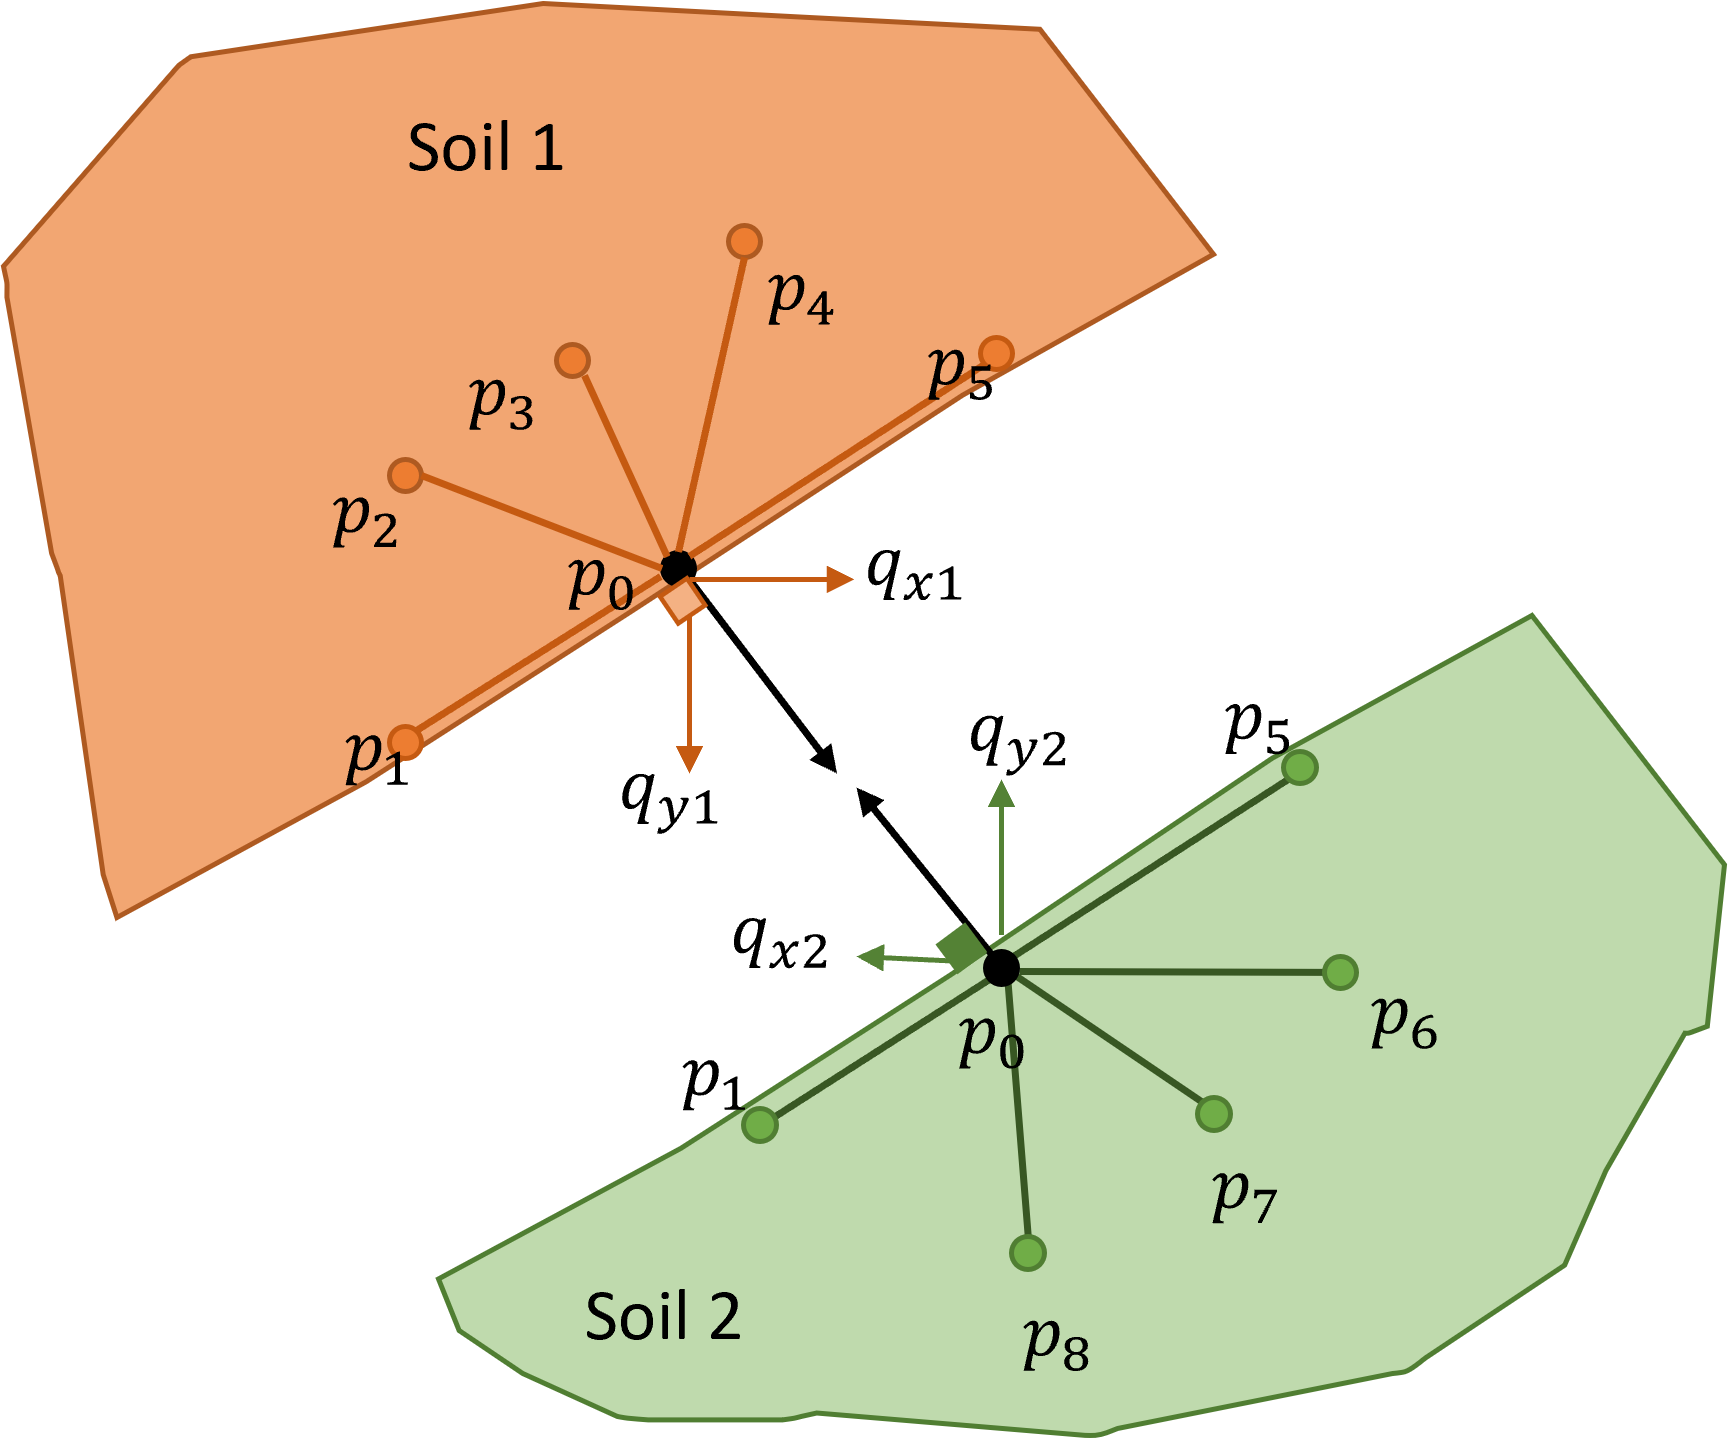
\includegraphics[width=.5\linewidth]{Balance1.png}
  \caption{Balance between  two layers }
  \label{fig1}
\end{figure}  

\begin{figure}[htb]
  \centering
  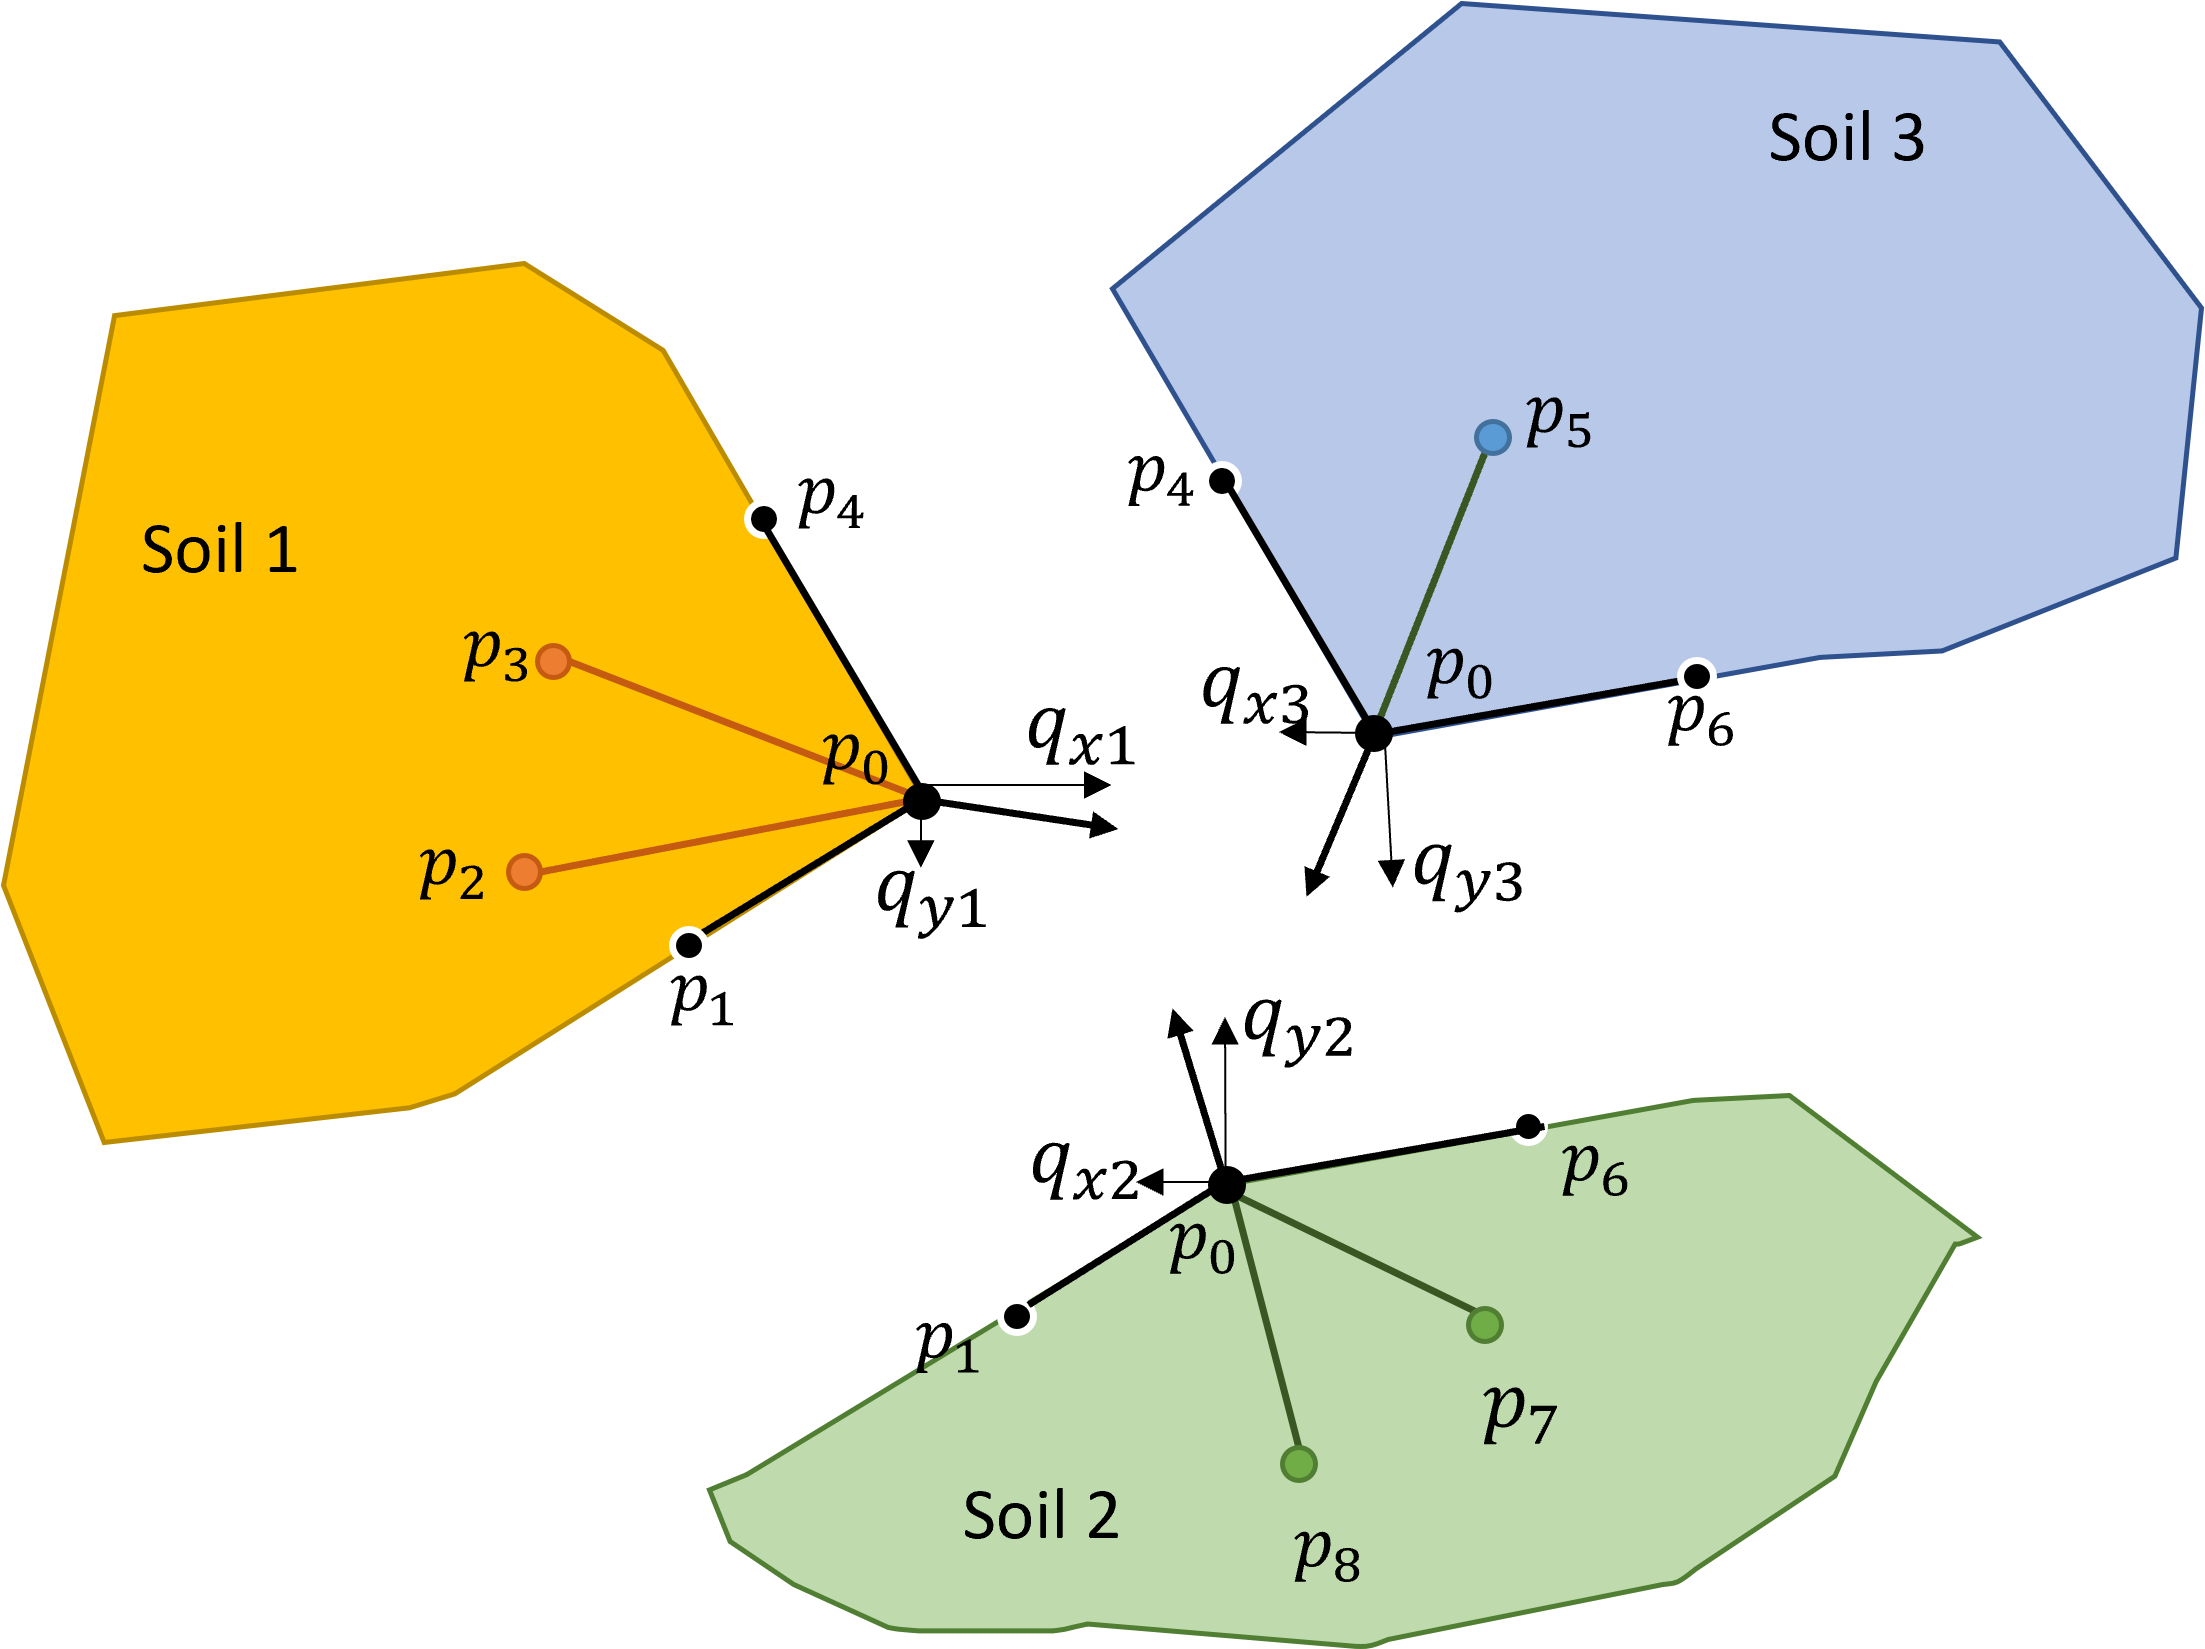
\includegraphics[width=.6\linewidth]{Balance2.png}
  \caption{Balance between  three layers}
  \label{fig2}
\end{figure} 


To apply the generalized finite difference method to the equation (\ref{eq10}), via equation (\ref{eq1}) and (\ref{eq2}), for the partial derivatives in direction $x$ and $y$, the coefficients $D$ and $E$ are taken as $k_{x_i}$ and $k_{y_i}$, respectively. Then, the balance on each boundary node can be posed as

\begin{equation}
  \sum_{i=1}^{nl} \left( k_{x_i} \sum_{j=1}^{nnl} \Gamma_j h(p_j) l_{x_i} +k_{y_i} \sum_{j=1}^{nnl} \Gamma_j h(p_j) l_{y_i} \right)
  =0,
  \label{eq11}
\end{equation}

where $nnl$ is the number of nodes on each layer $i$, and  $\Gamma_j$ is the $j-th$ coefficient of $h(p_j)$. It should be emphasized that the balance in the interface nodes given by Equation (\ref{eq11}) is the governing equation at the interface node, and therefore, it must be written as one row of the $H$ matrix. %There are no double or triple nodes.

Since one-sided derivatives are considered at the material boundary between two layers  (see Figure \ref{fig1} or \ref{fig2}), the calculus of the $\Gamma$ coefficients was made using the ghost node formulation proposed in \cite{chavez2021}. Thus, the normal derivative is formulated with an extra node $p_g$, localized in front of the interface. Then, the normal can be written as

\begin{equation}
  l_x\frac{\partial h}{\partial x}+l_y\frac{\partial h}{\partial y}=\frac{\partial h}{\partial n}(p_0)
  \approx \hat{\Gamma}_g h(p_g)+\sum_{l=0}^k\hat{\Gamma}_l h(p_l), 
  \label{eq12}
\end{equation}  

solving algebraically for $u(p_g)$ from the equation (\ref{eq12}), the equation (\ref{eq13}) is obtained. The resulting approximation is then substituted in the approximation of the differential equation (\ref{eq2}) to eliminate the ghost node, and the formulation for an interface node is completed.

\begin{equation}
 u(p_g)=\frac{1}{\hat{\Gamma}_g}\frac{\partial u}{\partial n}(p_0)-\sum_{l=0}^k\frac{\hat{\Gamma}_l}{{\hat{\Gamma}_g}} u(p_l).
 \label{eq13}
\end{equation}


\section{Implementation and validation of the balance formulation}

Implementing the interface balance in the generalized finite differences requires a previous thorough process for identifying all boundary nodes and the neighboring nodes on each one of the layers. The connection nodes $j$ on the $i$-th layer are associated with each node $p_0$ on the boundary. Then, the implementation makes a loop over all nodes to calculate the generalized finite difference coefficients for the differential equation selected (\ref{eq1}) to solve; if the chosen node is on the interface between layers, the coefficients of the balance of the layers are activated, and Equation (\ref{eq11}) is used as the governing equation. Afterward, the matrix of coefficients $H$ is assembled, and the problem is ready to be solved.    

Tests in interfaces of two and three materials were carried out to validate the above formulation.  Richards equation (\cite{fredlund2012}) for the case of stationary was chosen; it is derived from Darcy's law, and it can be written as

\begin{equation}
  \frac{\partial}{\partial x}\left(-k_x(s) \frac{\partial h}{\partial x} \right)+
  \frac{\partial}{\partial y}\left(-k_y(s) \frac{\partial h}{\partial y} \right)=0,
  \label{eq14}  
\end{equation}

where $k_x$ and $k_y$ are the coefficients of permeability, and, therefore, functions of the matrix suction ($s$) via volumetric water content $\theta_w$. differentiating the Equation (\ref{eq14}), the result is

\begin{equation}
  k_x(s) \frac{\partial^2 h}{\partial x^2} +k_y(s) \frac{\partial^2 h}{\partial y^2}+
  \frac{\partial k_x(s)}{\partial x} \frac{\partial h}{\partial x}+
  \frac{\partial k_y(s)}{\partial y} \frac{\partial h}{\partial y}=0.
  \label{eq15}  
\end{equation}

In this case, the van Genuchten-Mualem equation was used to model the water unsaturated permeability function; it is expressed as

\begin{equation}
k(\theta_{w})=k_{sat}\sqrt{\theta_{w}}(1-(1-\theta_{wn}^{1/m}))^2
\label{eq16}  
\end{equation}

where $m$ is a fitting parameter, for this case, the $\theta_w$ value is obtained with the following equation.  

\begin{equation}
\theta_{w}=\frac{1}{((\alpha s)^n+1)^m}
\label{eq17}  
\end{equation}


due to van Genuchten, where $m$ and $n=1/m$ are adjustment parameters.

%Then after the simulation of the steady confined seepage in a foundation dam. 

In the case of saturated soil, the governing differential equation for steady-state seepage through a porous medium is the Laplace equation, which can be expressed as

\begin{equation}
  \nabla^2 h=0,
  \label{eq18}  
\end{equation}

where $\nabla^2$ is the Laplacian operator (\cite{desai2013advanced}).

\subsection{Solution of Laplace equation in benchmark problems}

This subsection presents the tests made in interfaces of two and three layers to validate the above formulation. The first test is a rectangle with a vertical interface, the second a rectangle with an inclined interface, and the third a square with three layers. %The results for the simulation of the steady confined seepage in a foundation dam with a sheet pile are presented.      

The mesh points for the first validation case are presented in Figure \ref{fig3}; it is a rectangle of 2 units of length and 1 unit of width, with a vertical interface at the middle of the length. It has two layers: the points in blue and orange, and the purple points represent the interface. The Dirichlet boundary conditions are marked with green nodes; the left part was set to 10, and the right one to zero. The red nodes represent the Neumann boundary conditions, where the value $\partial h/\partial n=0$ was set. The coefficients of permeability were set to 5 and 1, respectively. The total number of nodes is 231.  

The results are shown in the Figure (\ref{fig4}). We can see the vertical equipotential lines, and the distance between them is greater on the left side (k=5) and lower to the right (k=1); the low permeability produces more significant energy loss. A slope change can be noticed in the interface between the two. The same problem using the same mesh was solved in a 2D Finite Element Program considering a linear triangular element to validate the results. The results of a longitudinal section are compared in Figure (\ref{fig5}). The values of the total heads are practically equal. For the direct comparison between the FEM and GFDM, all results are presented using the norm $L_{RMSE}$ (Root Mean Square Error), defined as  

\begin{equation}
  L_{RMSE}= \sqrt{\frac{1}{n}\sum(h_{FEM}-h_{GFDM})^2}.
  \label{eql2}
\end{equation}

where $n$, is the number of nodes.

The norm $L_{RMSE}$ between the interface nodes is 3.47e-14, and 2.606e-14 considering all the nodes. The error values are significatively low, which implies a good agreement between the two methods for this case.  

\begin{figure}[htb]
  \centering
  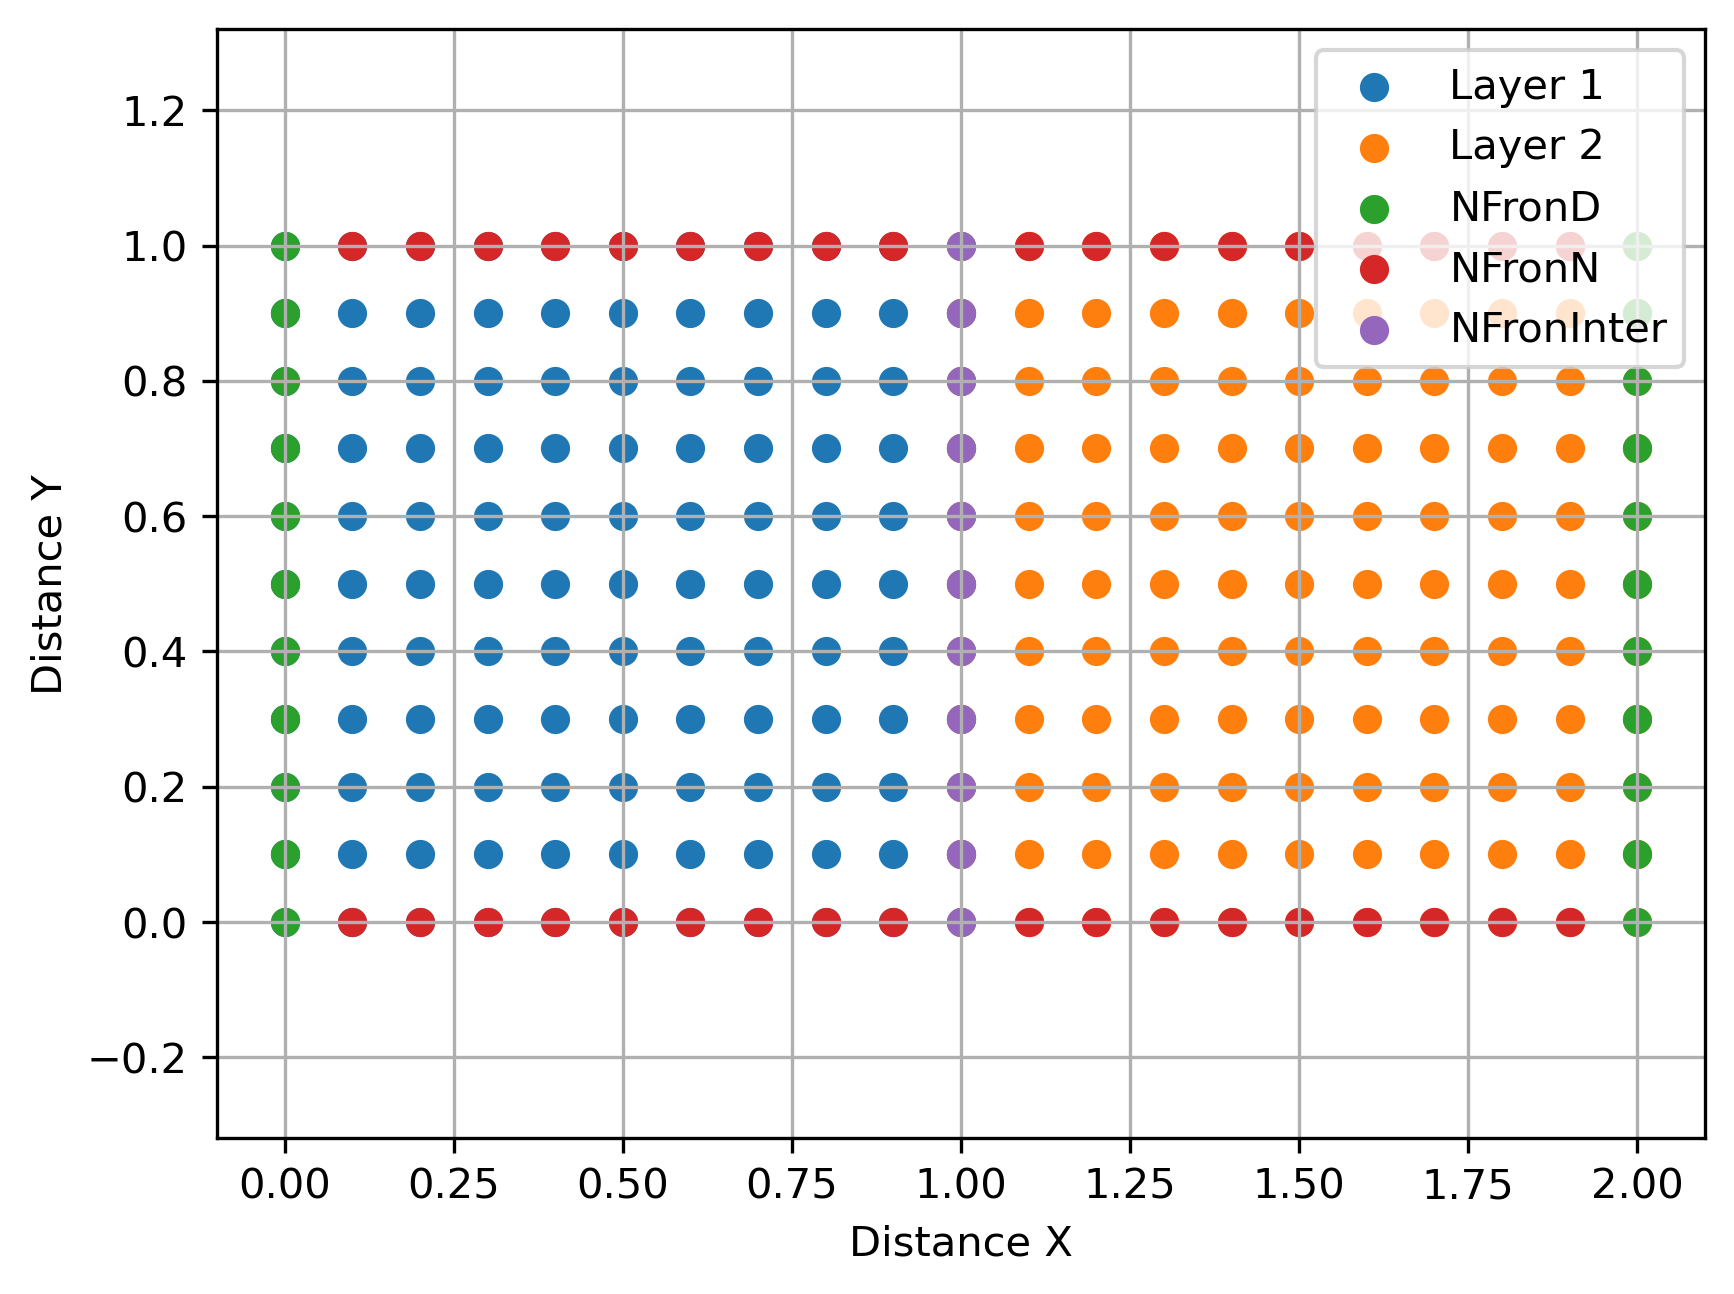
\includegraphics[width=0.8\textwidth]{FigSimpleHor1.png}
  \caption{Mesh for a simple problem interface}
  \label{fig3}
\end{figure}
 
\begin{figure}[htb]
  \centering
  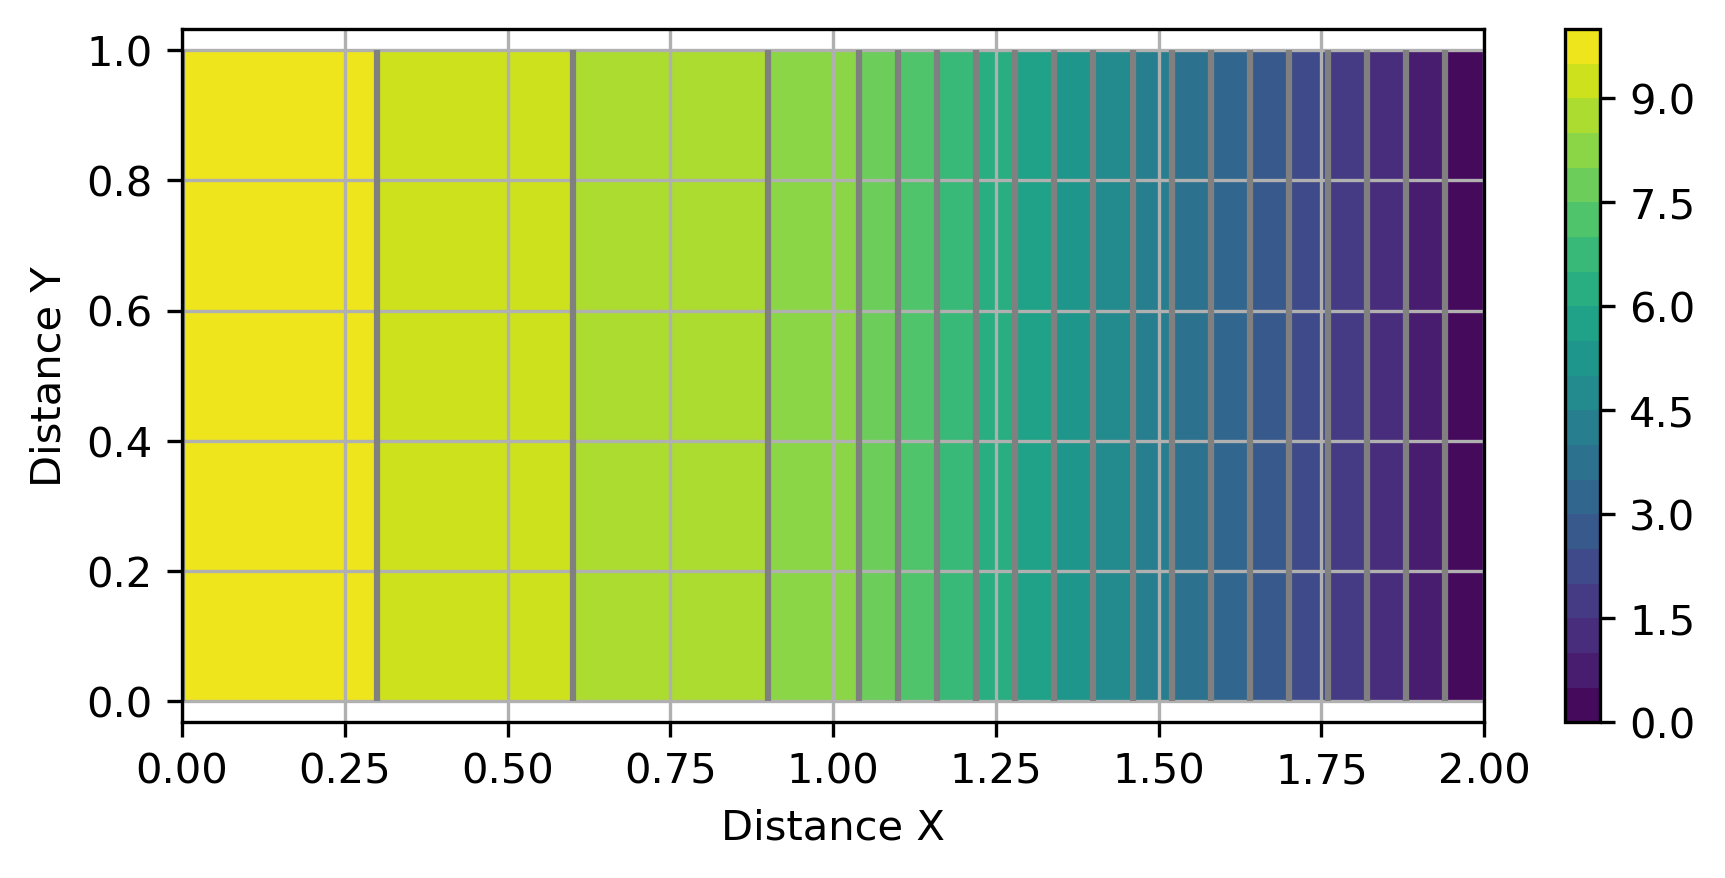
\includegraphics[width=0.8\textwidth]{FigSimHor1R.png}
  \caption{Results for a simple problem interface}
  \label{fig4}
\end{figure}

\begin{figure}[htb]
  \centering
  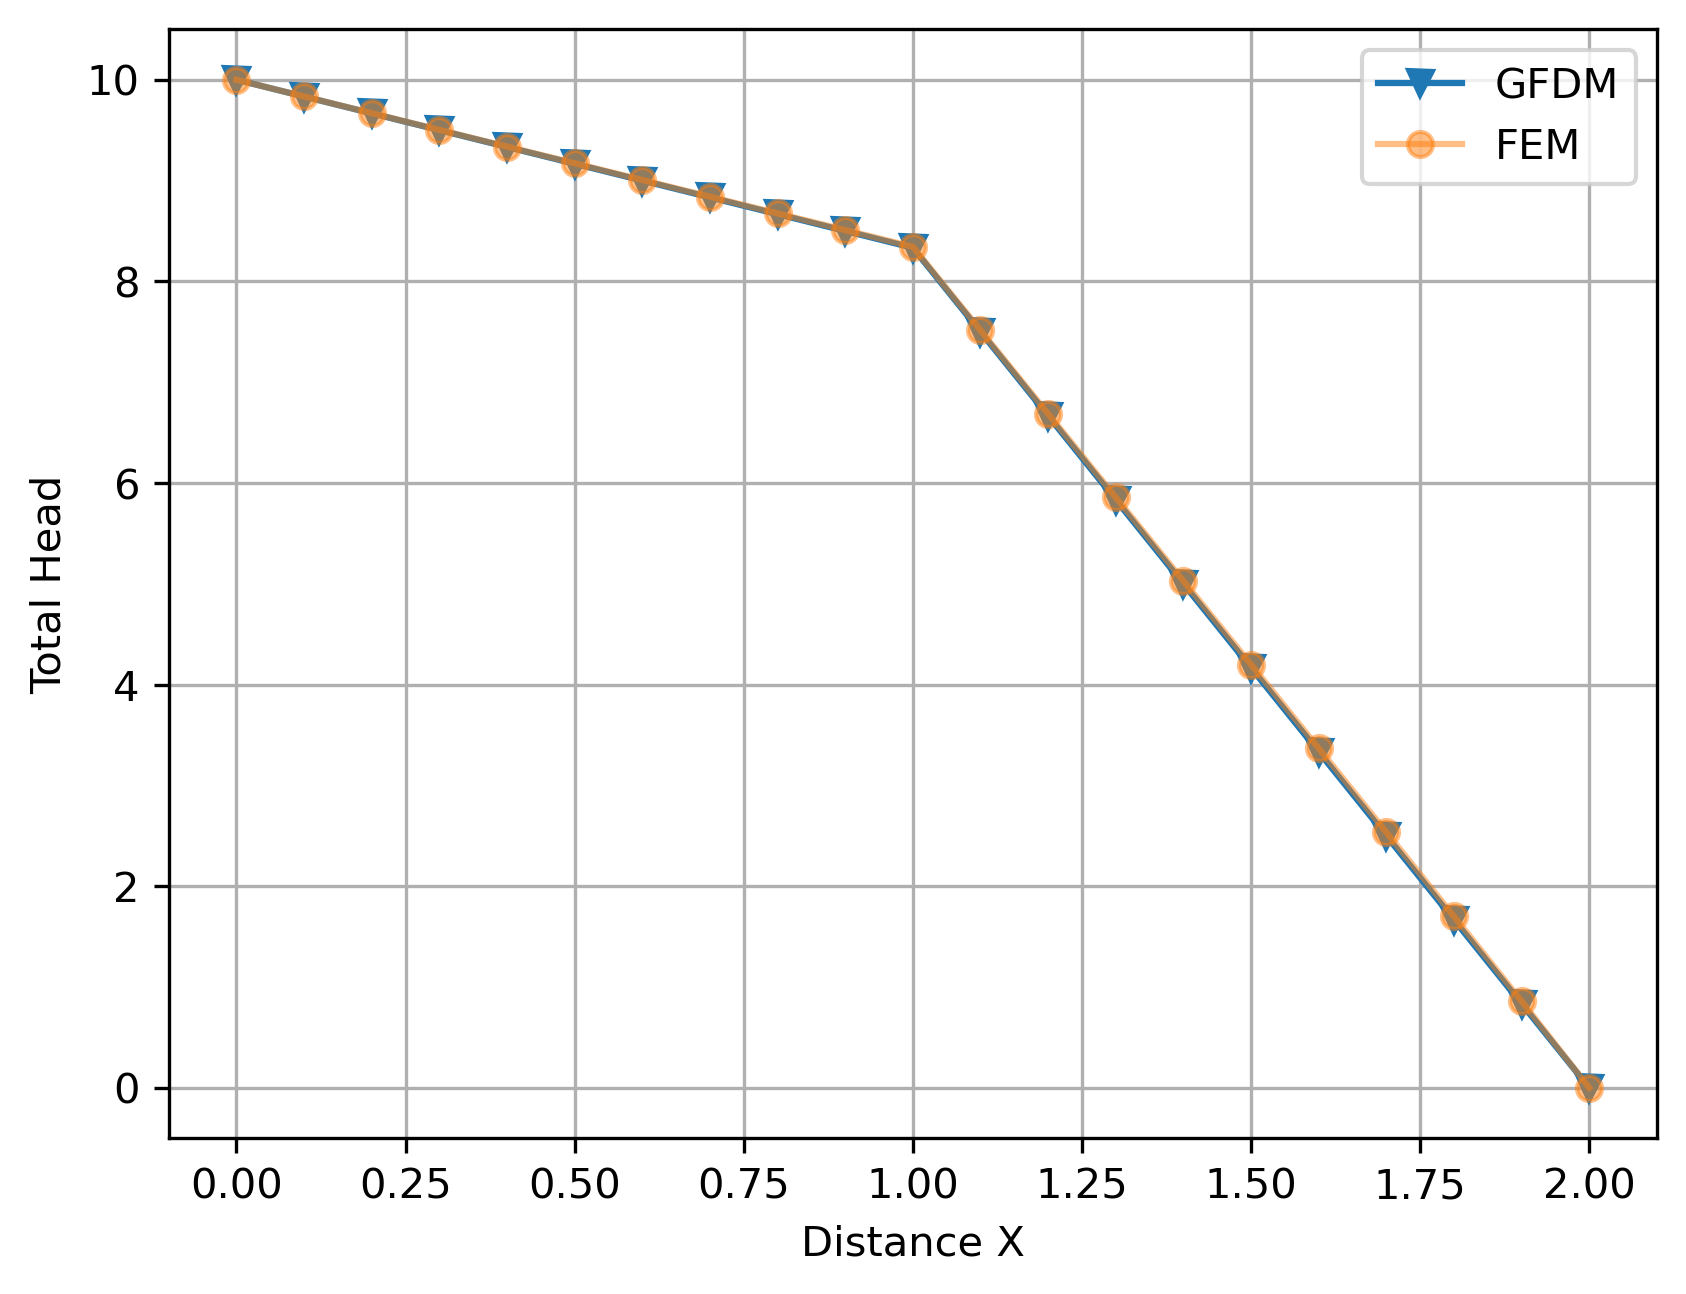
\includegraphics[width=0.6\textwidth]{CompaCS1.png}
  \caption{Results for a simple problem interface}
  \label{fig5}
\end{figure}

Another test considered the interface with an inclination (see Figure \ref{fig6}). In this case, the figure was rotated 90 degrees. The permeabilities were the same as in the previous example for each layer, and the number of nodes was 265; the results are shown in Figure (\ref{fig7}). The equipotential lines are more separated in the first layer (k=5) than in the second layer (k=1). In this case, there is a difference between the solution with GFDM and FEM in the layer with low permeability. To appreciate the difference, the values of the total head at the left-hand side and right-hand side (vertical boundaries) were plotted; they are presented in Figure (\ref{fig8}). The figure illustrates the total head on the left and right side; the results show a visible difference between the solution for GFDM and FEM on the right-hand side. The $L_{RSME}$ norm considering all nodes is 0.057, and at the interface is 0.094. In this case, the solution is different but with an accurate approximation.   

\begin{figure}[htb]
  \centering
  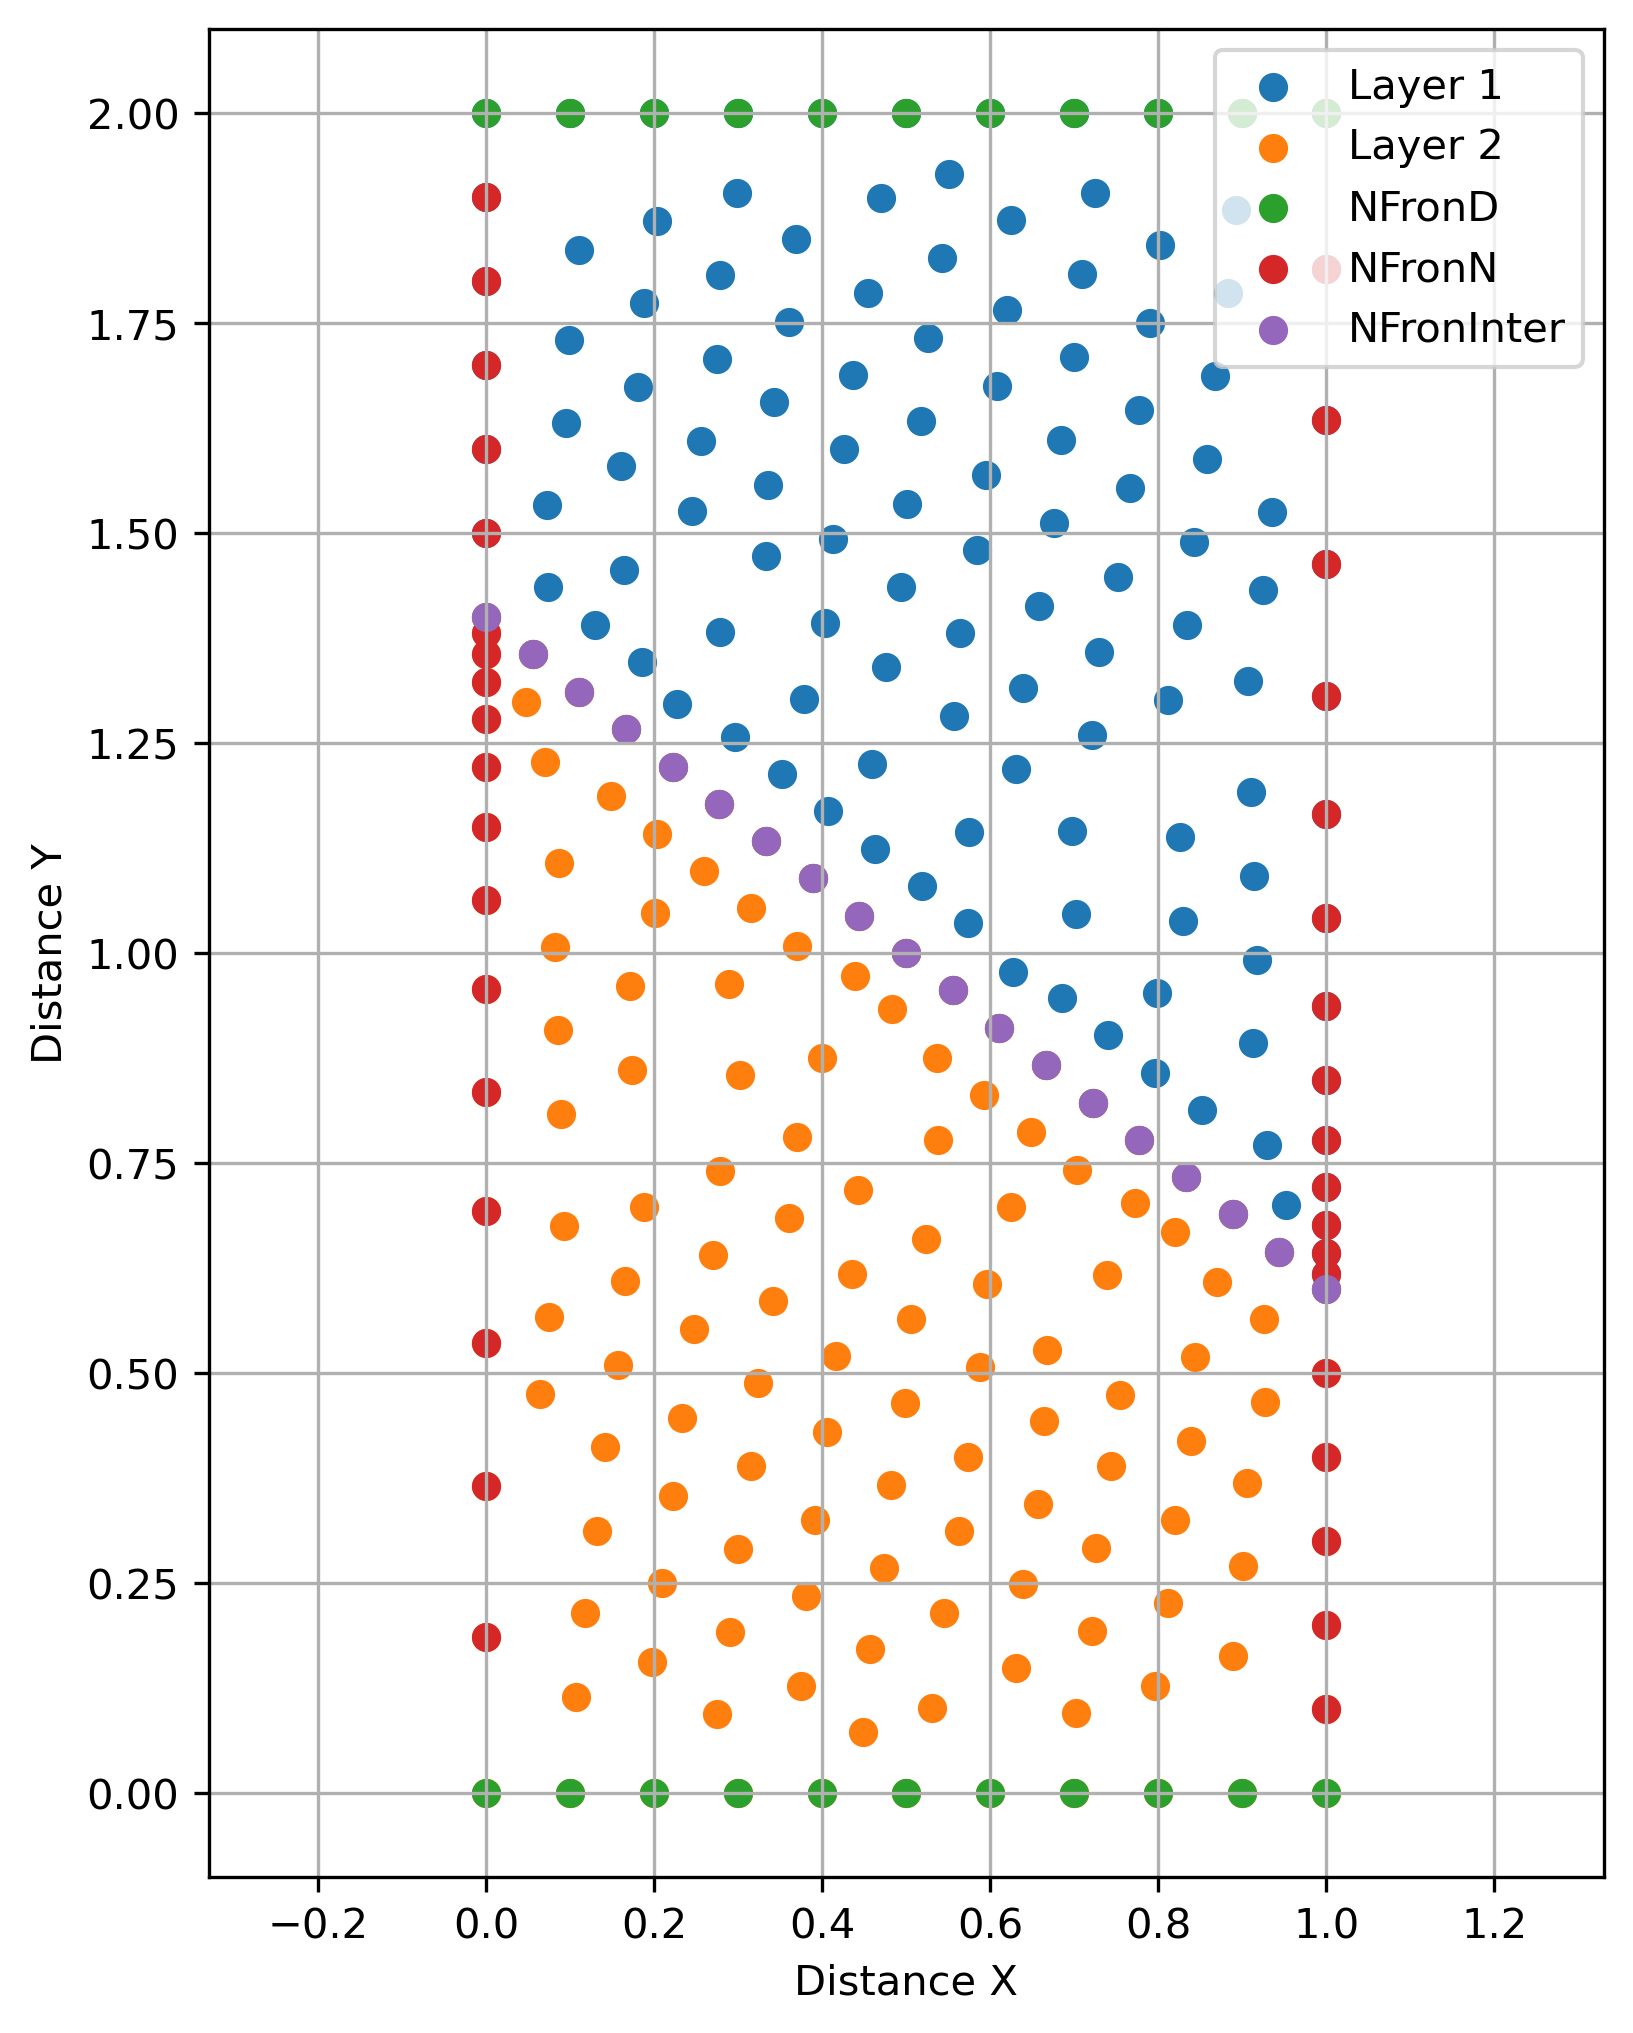
\includegraphics[width=0.6\textwidth]{FigSimMshVer1.png}
  \caption{Nodes used for the inclined interface problem}
  \label{fig6}
\end{figure}

\begin{figure}[htb]
  \centering
  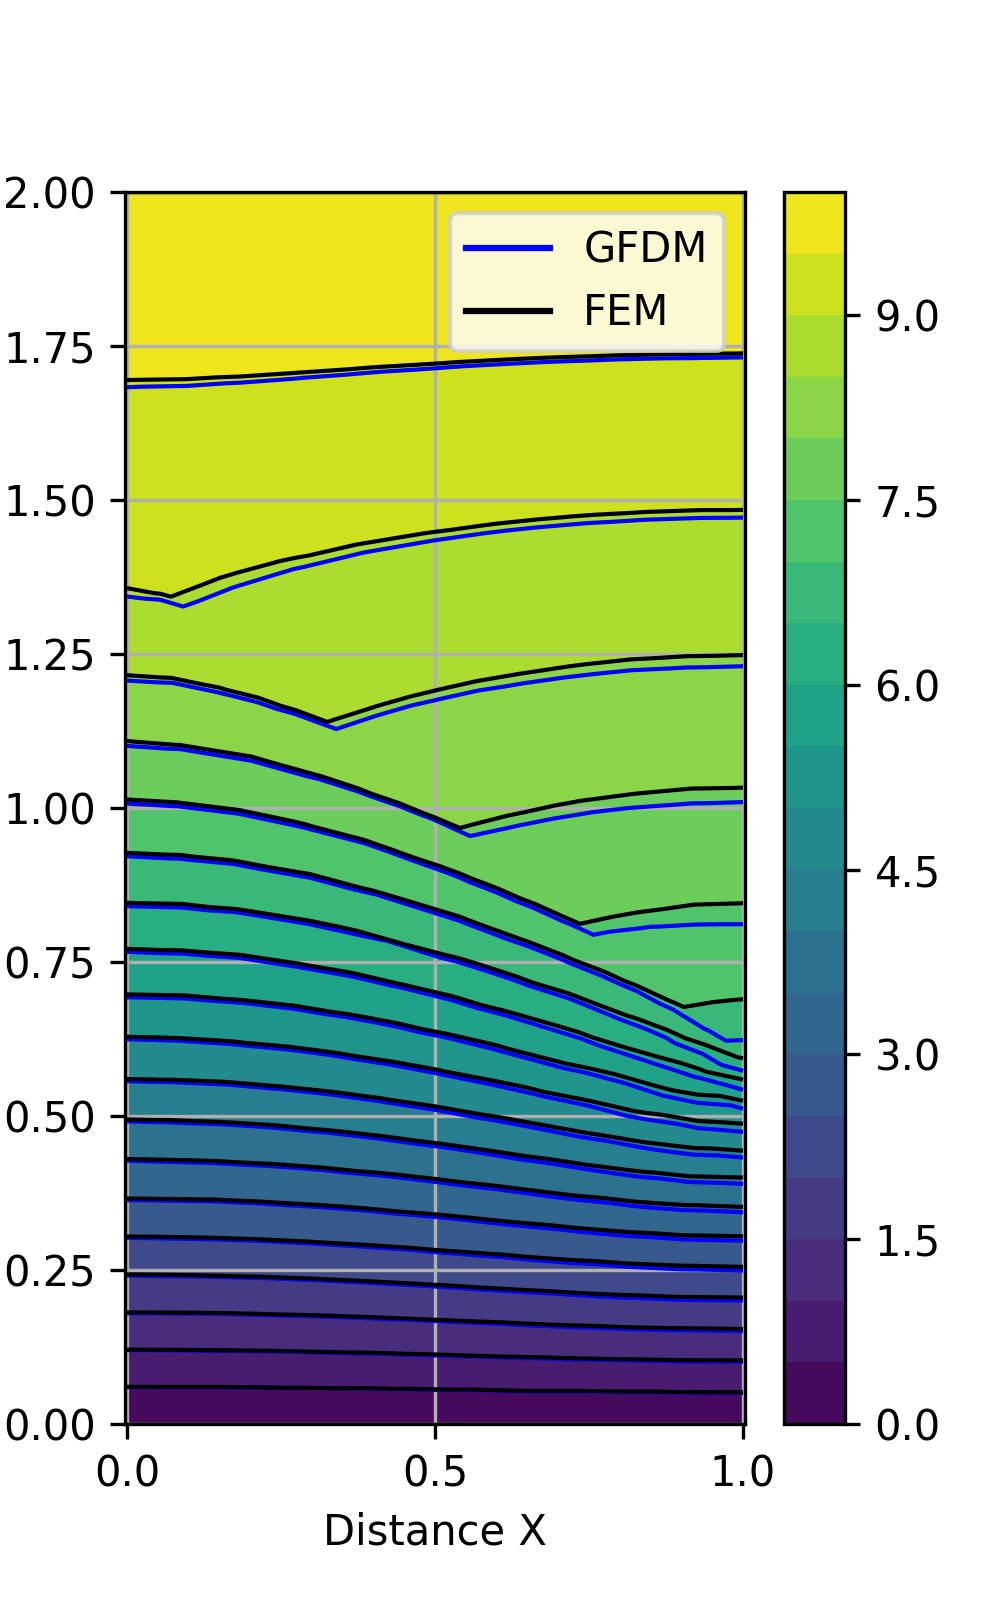
\includegraphics[width=0.6\textwidth]{Caso2Compara.png}
  \caption{Equipotential lines for inclined interface problem}
  \label{fig7}
\end{figure}

\begin{figure}[htb]
  \centering
  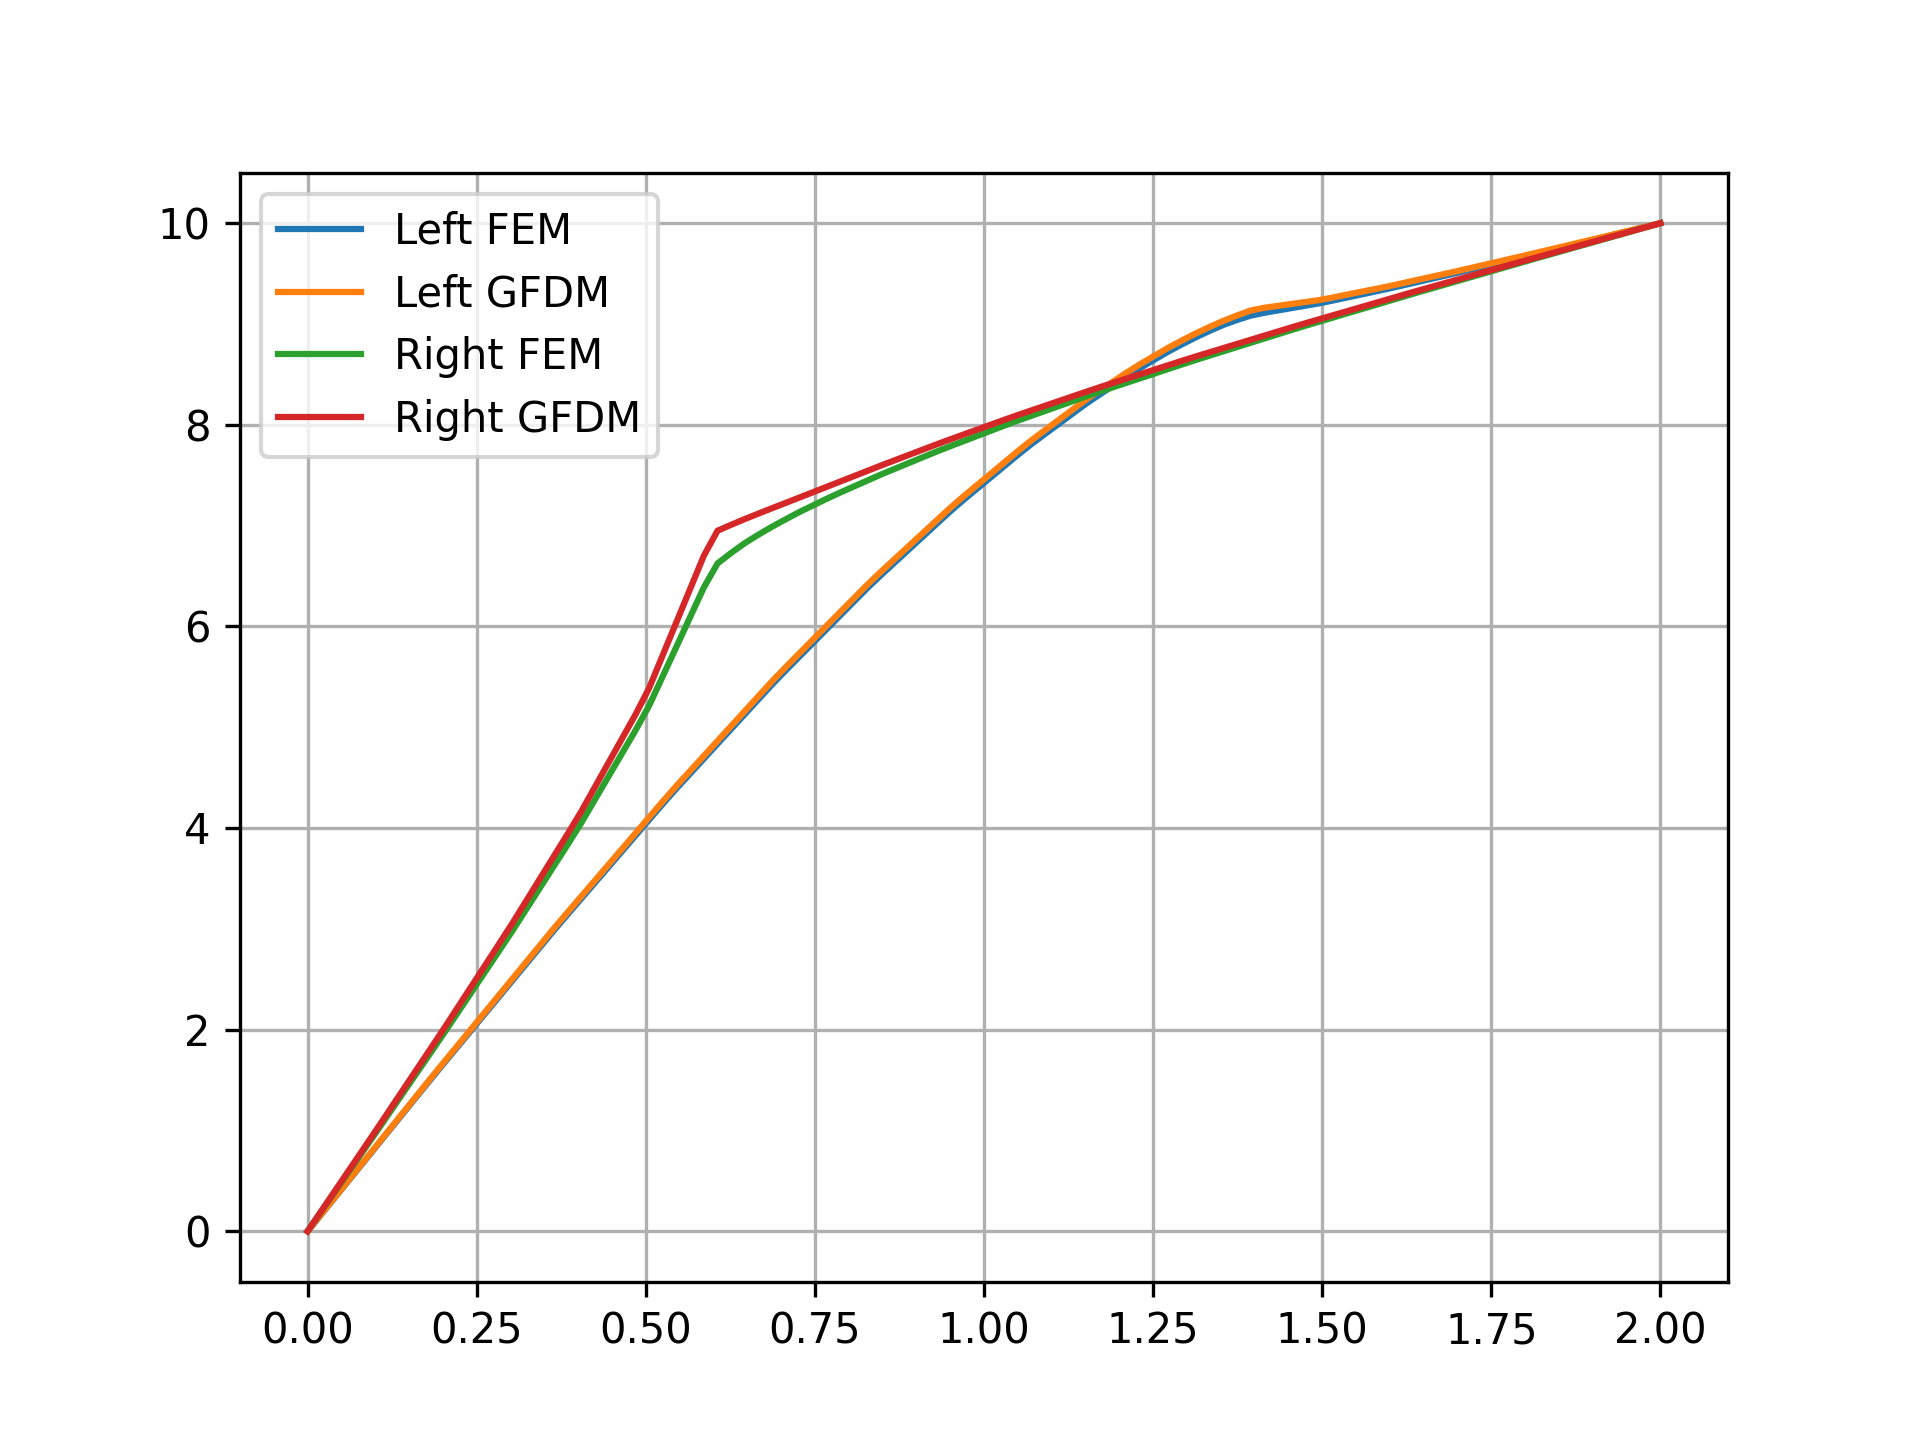
\includegraphics[width=0.8\textwidth]{Caso2CompaCS3.png}
  \caption{Results for a simple problem interface}
  \label{fig8}
\end{figure}

The third test case is a square with three layers and different permeability coefficients (1, 100, and 50). Figure (\ref{fig:93C}) shows the mesh of points with the different regions and boundaries. The left and right boundaries have Dirichlet conditions set to 10 and 20, respectively, and the upper and lower are for Neumann ones ($\partial h/\partial n=0$). In the center of the square is the point that divides the three layers; in this case, the balance for this point is done as is explained in Figure (\ref{fig2}). Figure (\ref{fig:10C}) illustrates the solution for the three layers case; the isolines in blue are for the GFDM, and the lines in black for FEM using triangles with three nodes, both methods with the same mesh. The solution is nearly the same; there is a slight separation for the iso-lines in the case of the layer with the lower permeability (layer 2). The $L_{RMSE}$ norm in the nodes on the interface is 0.042 and, in general, is 0.0326.  

We can conclude, taking all nodes into account, that there is less difference than when considering only the nodes in the interface. Additionally, in regions with low permeability, the equipotential lines are more widely spaced, which leads to increased errors.

\begin{figure}[htb]
  \centering
  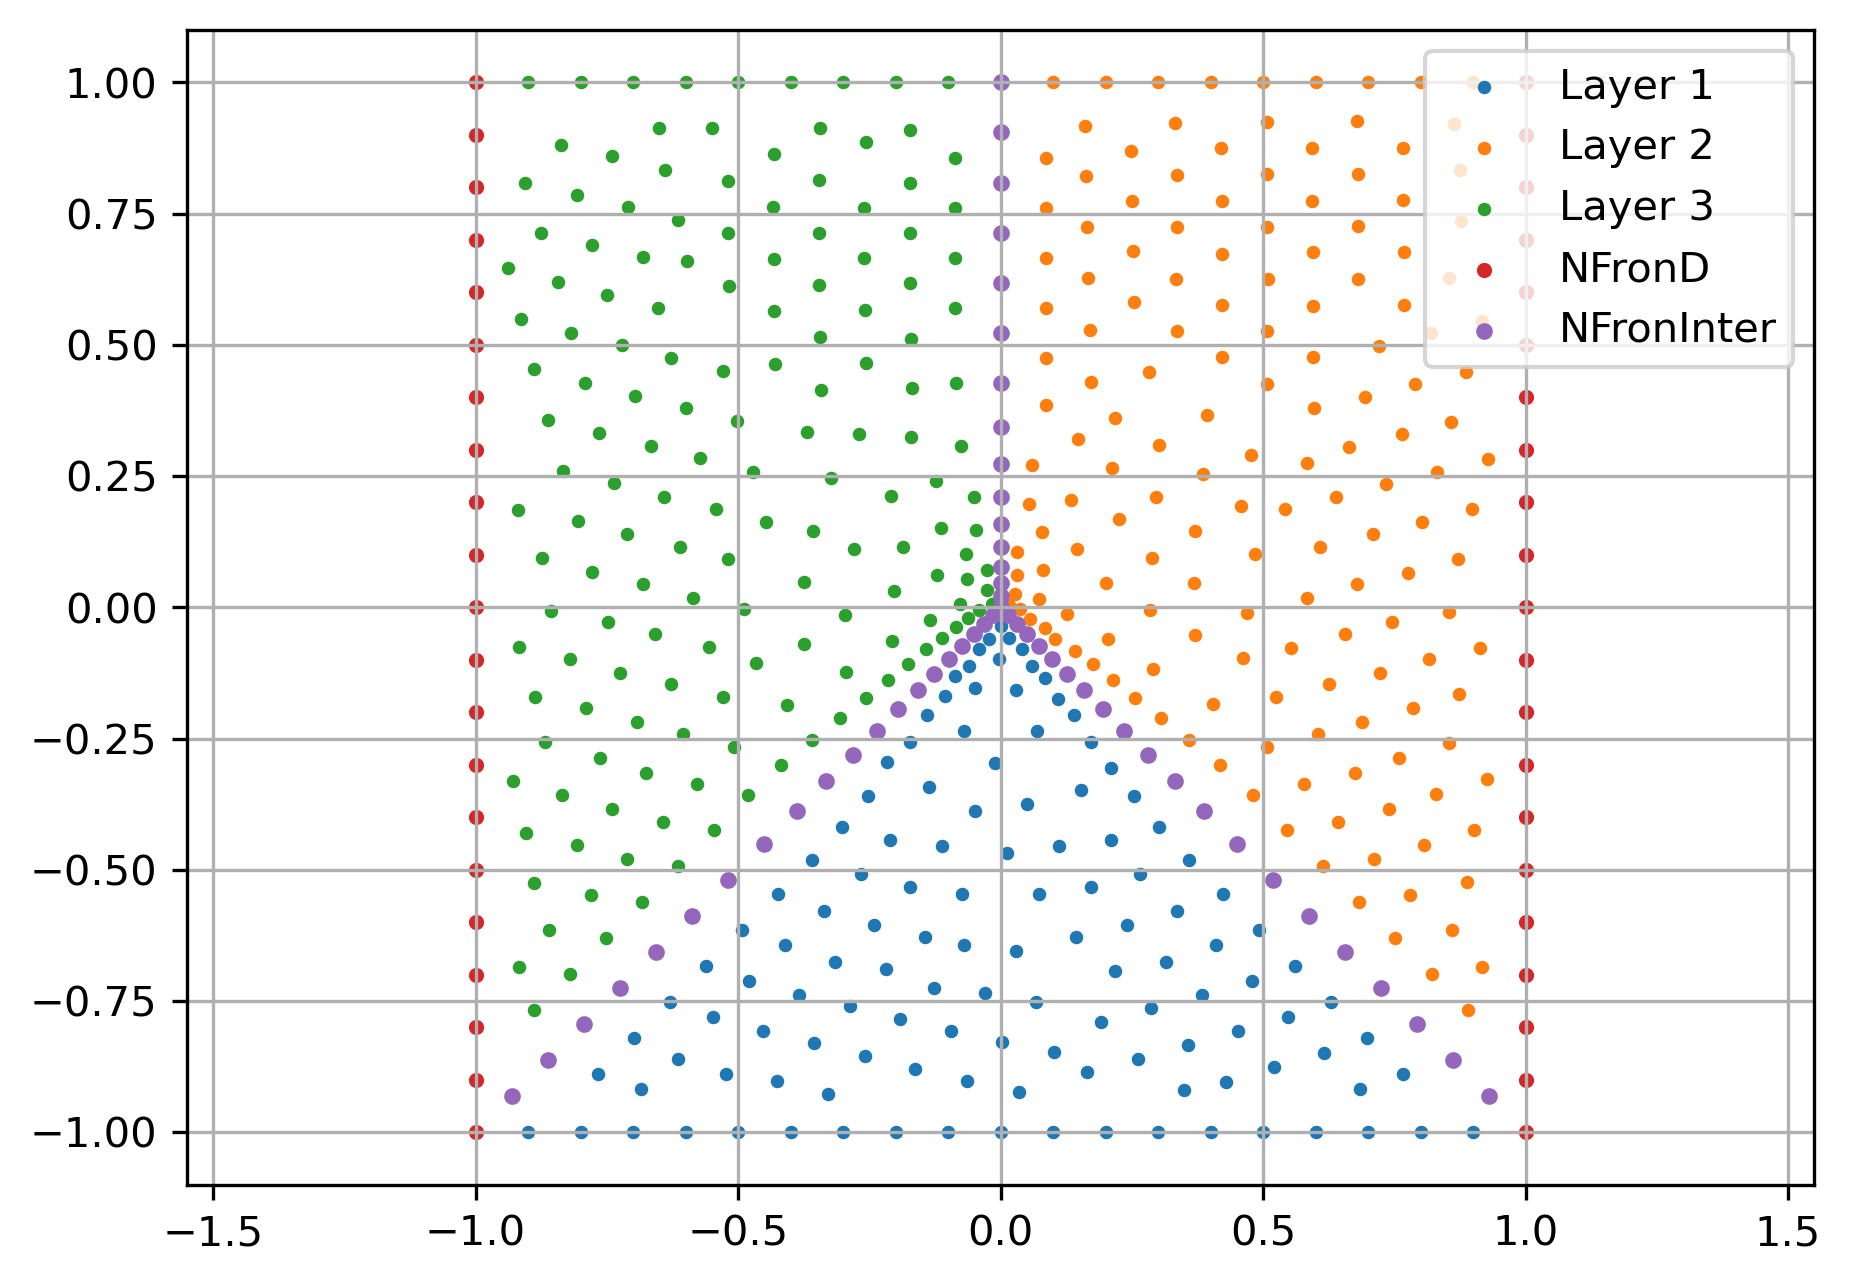
\includegraphics[width=0.8\textwidth]{FigFronMsh3.png}
  \caption{Mesh of points for the square with three layers}
  \label{fig:93C}
\end{figure}

\begin{figure}[htb]
  \centering
  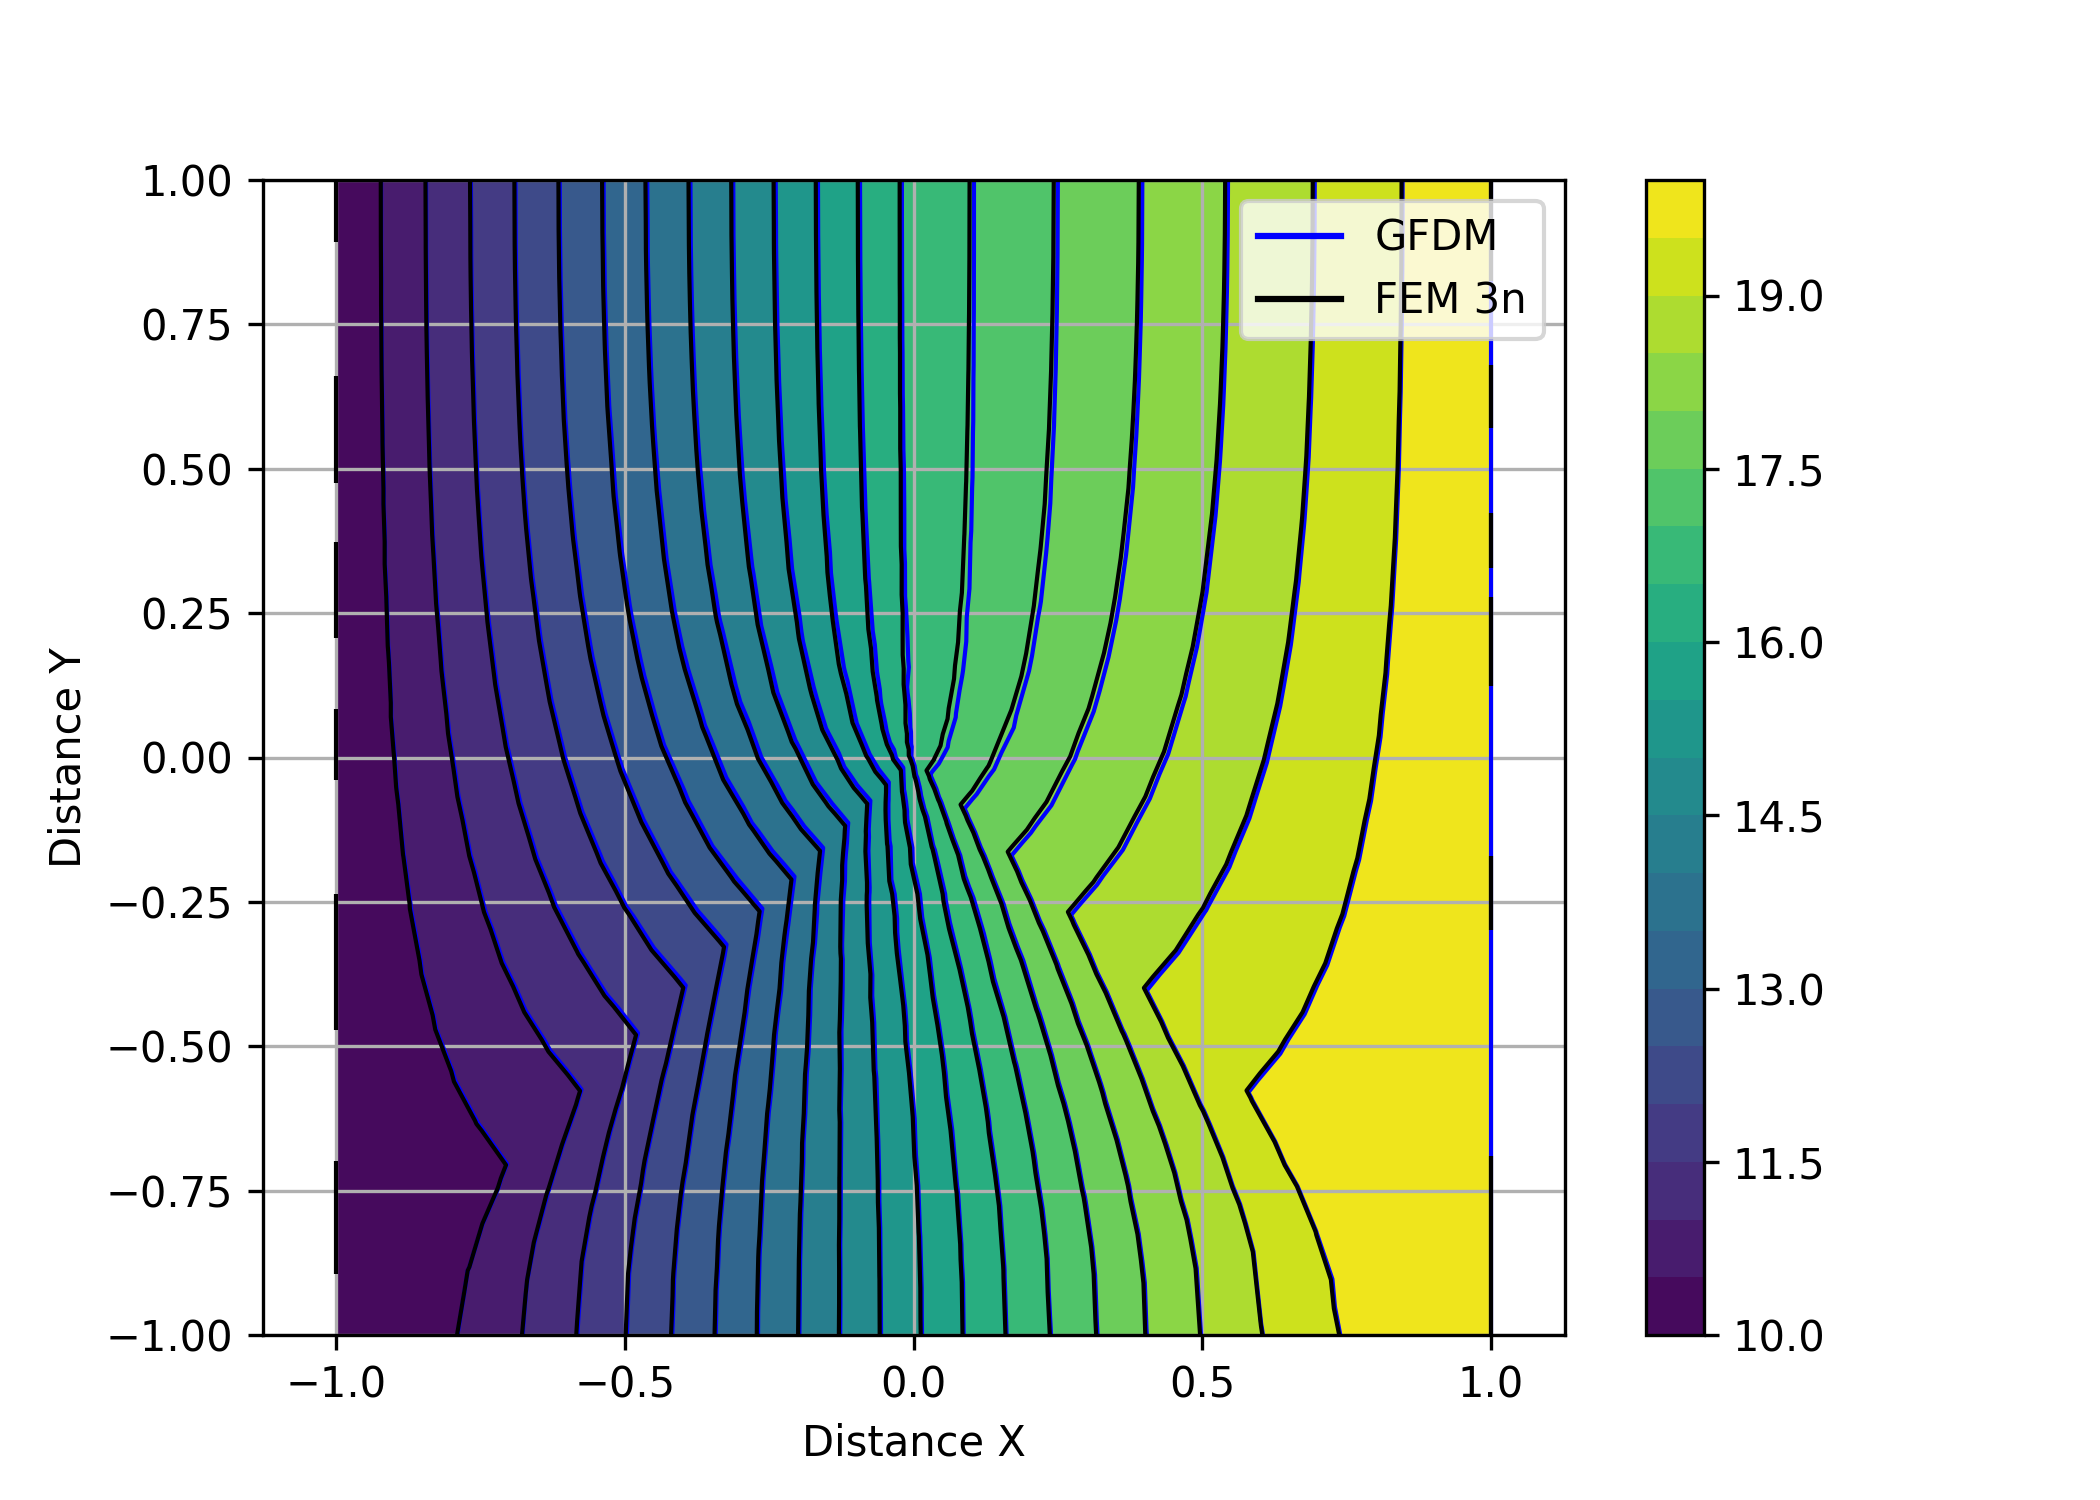
\includegraphics[width=0.8\textwidth]{Caso3Compara.png}
  \caption{Solution for the square with three layers}
  \label{fig:10C}
\end{figure}

\subsection{Solution of problems of groundwater flow}

The previous cases helped prepare the code to solve more complex problems. This section presents the solution to geotechnical problems of groundwater flow. The cases are the classic confined seepage in a dam foundation with two layers and the case of a dam with two and five layers.          

\subsubsection{Confined seepage in the  foundation dam}

A confined seepage in the foundation dam with a sheet pile was chosen to test the formulation in a saturated medium with two layers. The mesh with 1120 nodes is presented in Figure (\ref{fig:112c}); the orange nodes are for layer one, and the blue nodes are for layer two.  The Neumann boundary conditions are as follows: in the left, right, and bottom sides are $\frac{\partial h}{\partial n}=0$, and in the middle upper are applied the same conditions (red nodes). The Dirichlet boundary conditions are sketched in green; on the left upper side, a total head of 30 $m$ was applied; on the right upper side, a total head of 22 $m$; the permeabilities are 5 and 20 for layers one and two.  

The solution is presented in Figure (\ref{fig:12Com}). The solution for GFDM is shown in blue, and in black is the solution for FEM with linear triangular elements. The solution matches very well, except in the area downstream to the right of the sheet pile. The $L_{RMSE}$ norm for the interface for this case is 0.028 and, generally, for all nodes, is 0.031. If the FEM problem is solved with six node elements and the same mesh, the solution of the FEM case is more approximated to the GFDM solution, as shown in the Figure (\ref{fig:13}). The values of the $L_{RMSE}$ norm are 3.27e-3 and 3.47e-4 for the interface and for all nodes, respectively. This suggests that the GFDM yields an accurate approximation in this case.   

\begin{figure}[htb]
  \centering
  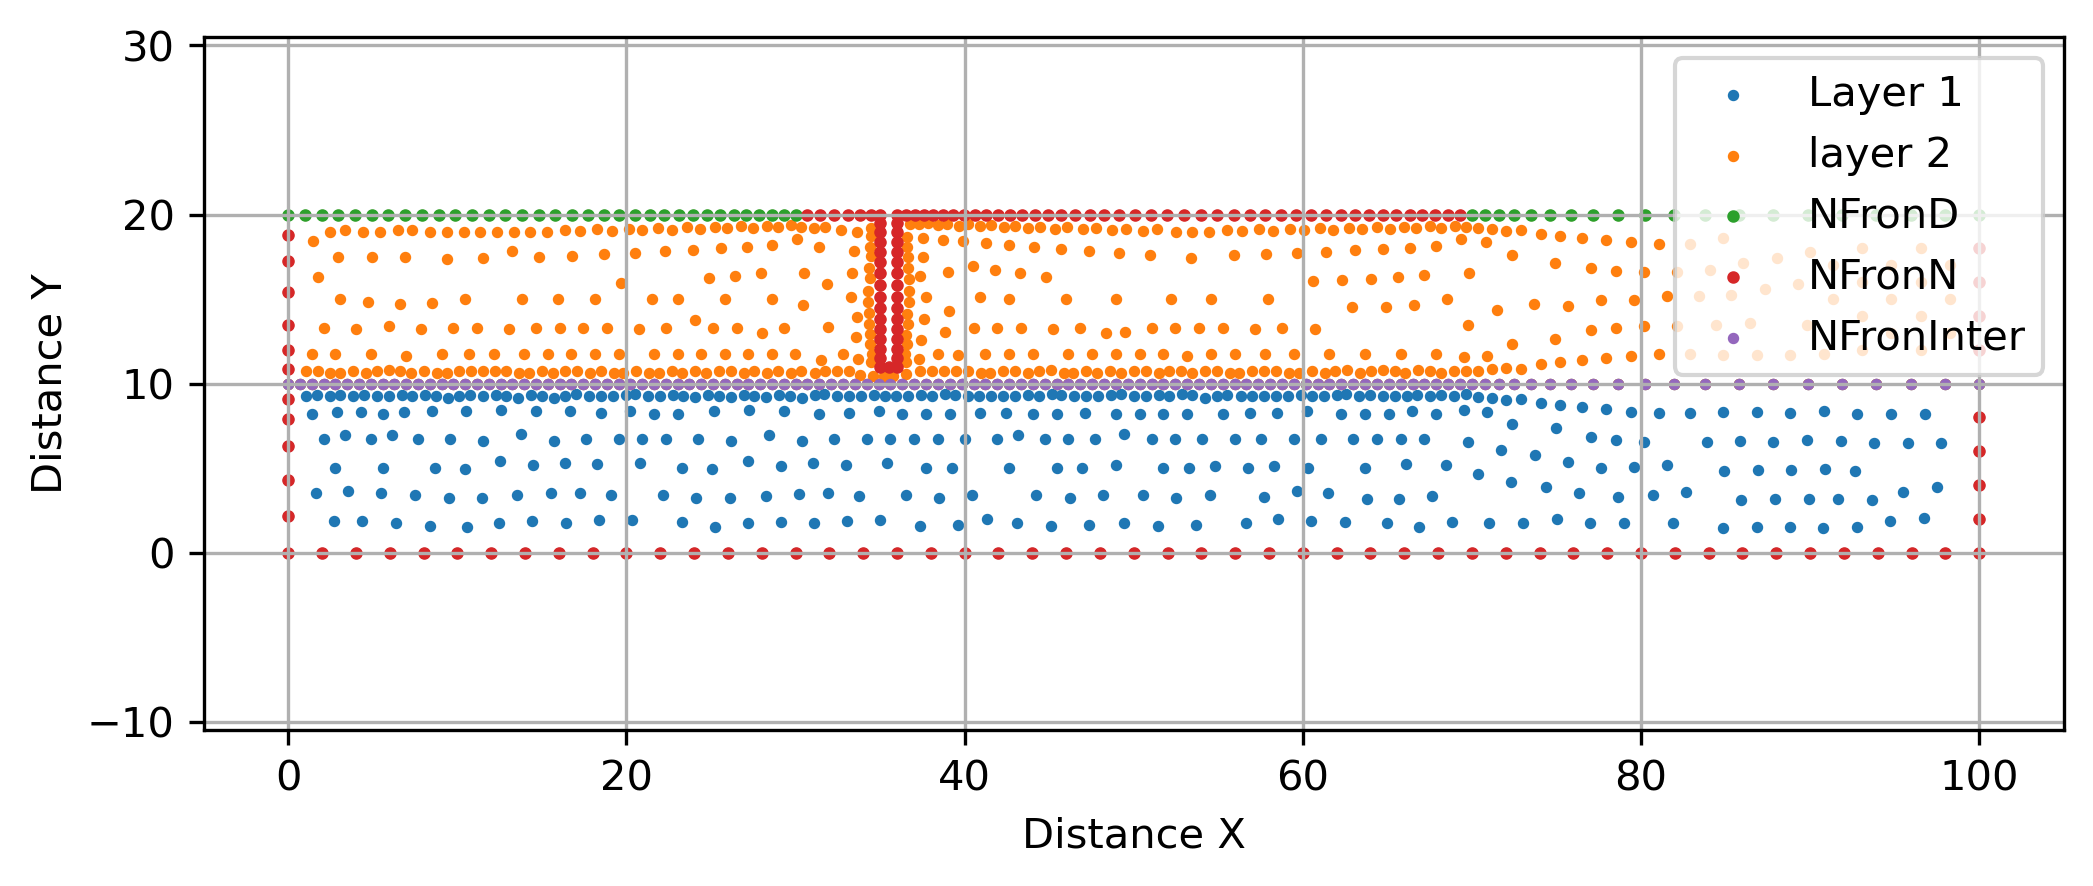
\includegraphics[width=0.8\textwidth]{FigDam1.png}
  \caption{Mesh for confined seepage in a foundation dam}
  \label{fig:112c}
\end{figure}

\begin{figure}[htb]
  \centering
  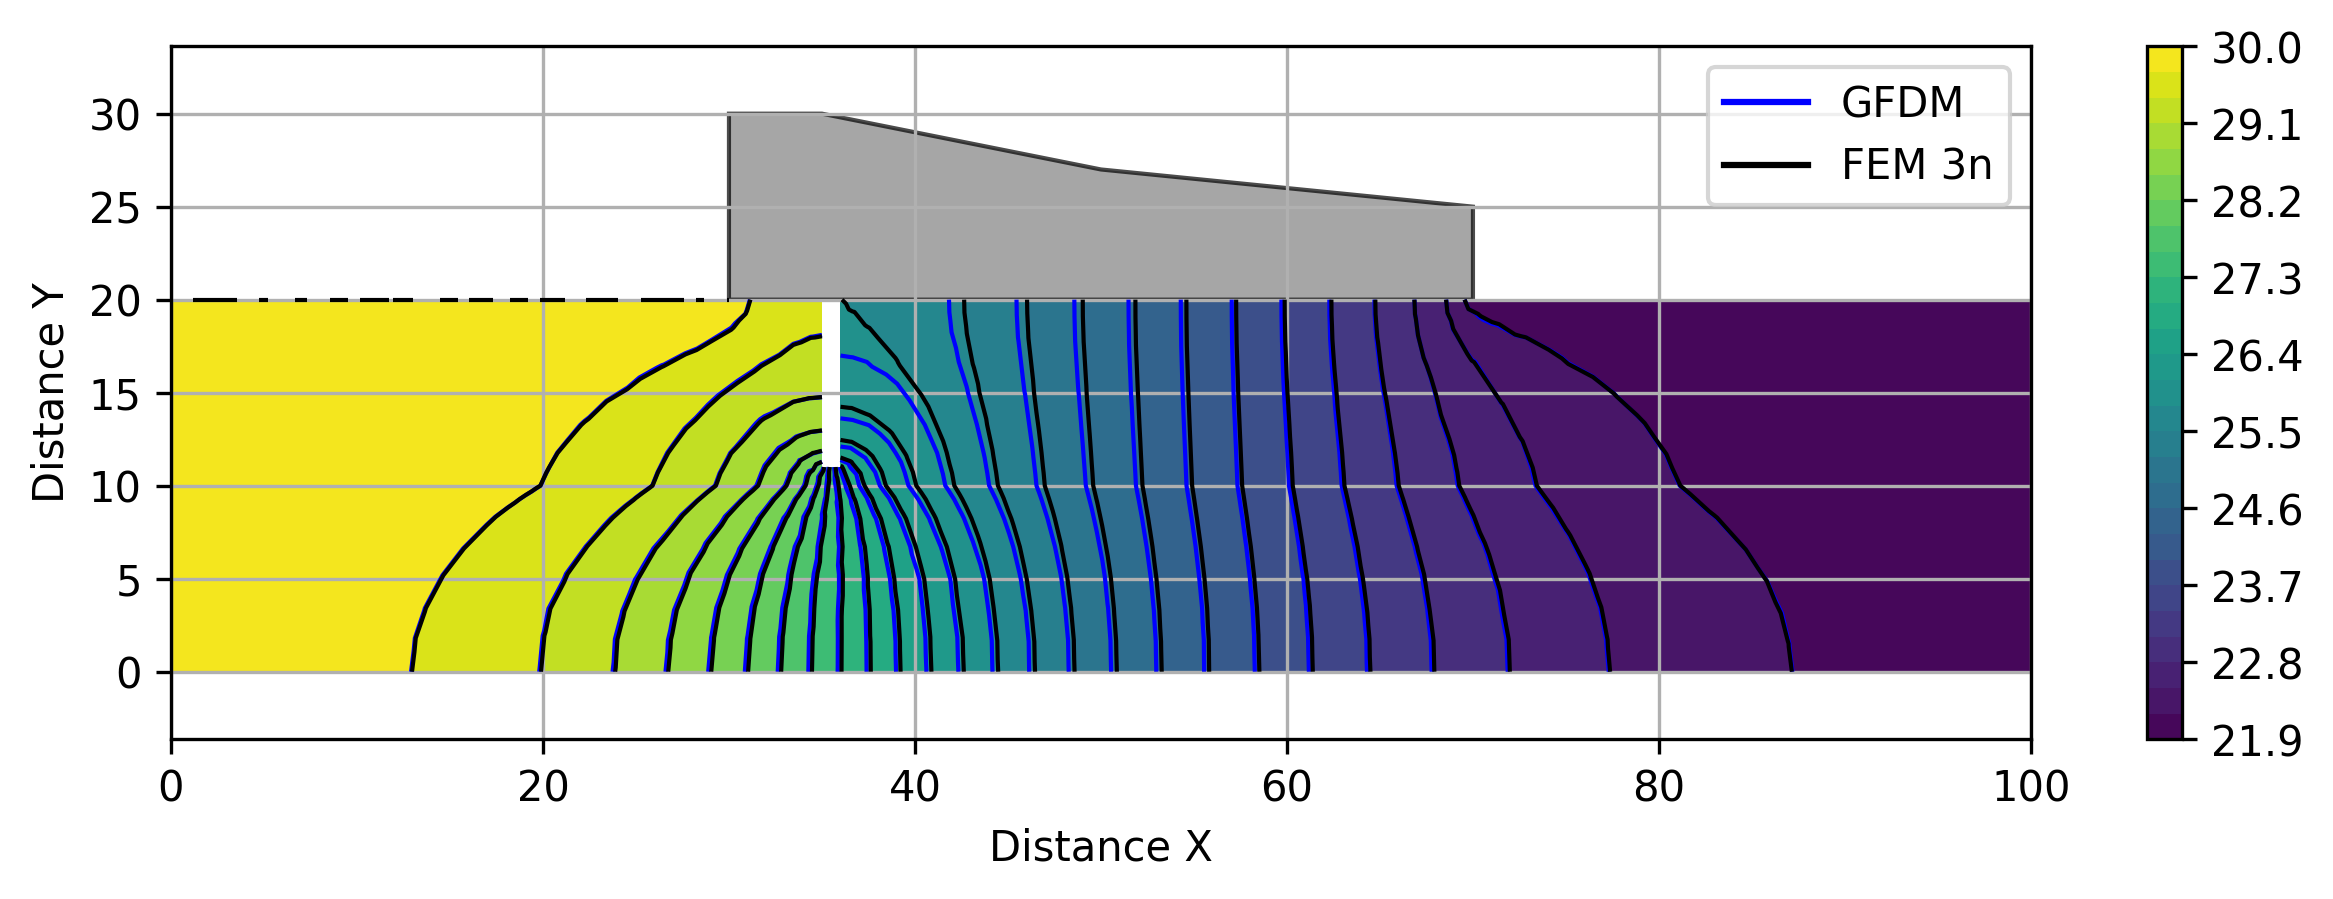
\includegraphics[width=0.95\textwidth]{Presa1Compara.png}
  \caption{Results for confined seepage in a foundation dam with the same mesh}
  \label{fig:12Com}
\end{figure} 

\begin{figure}[htb]
  \centering
  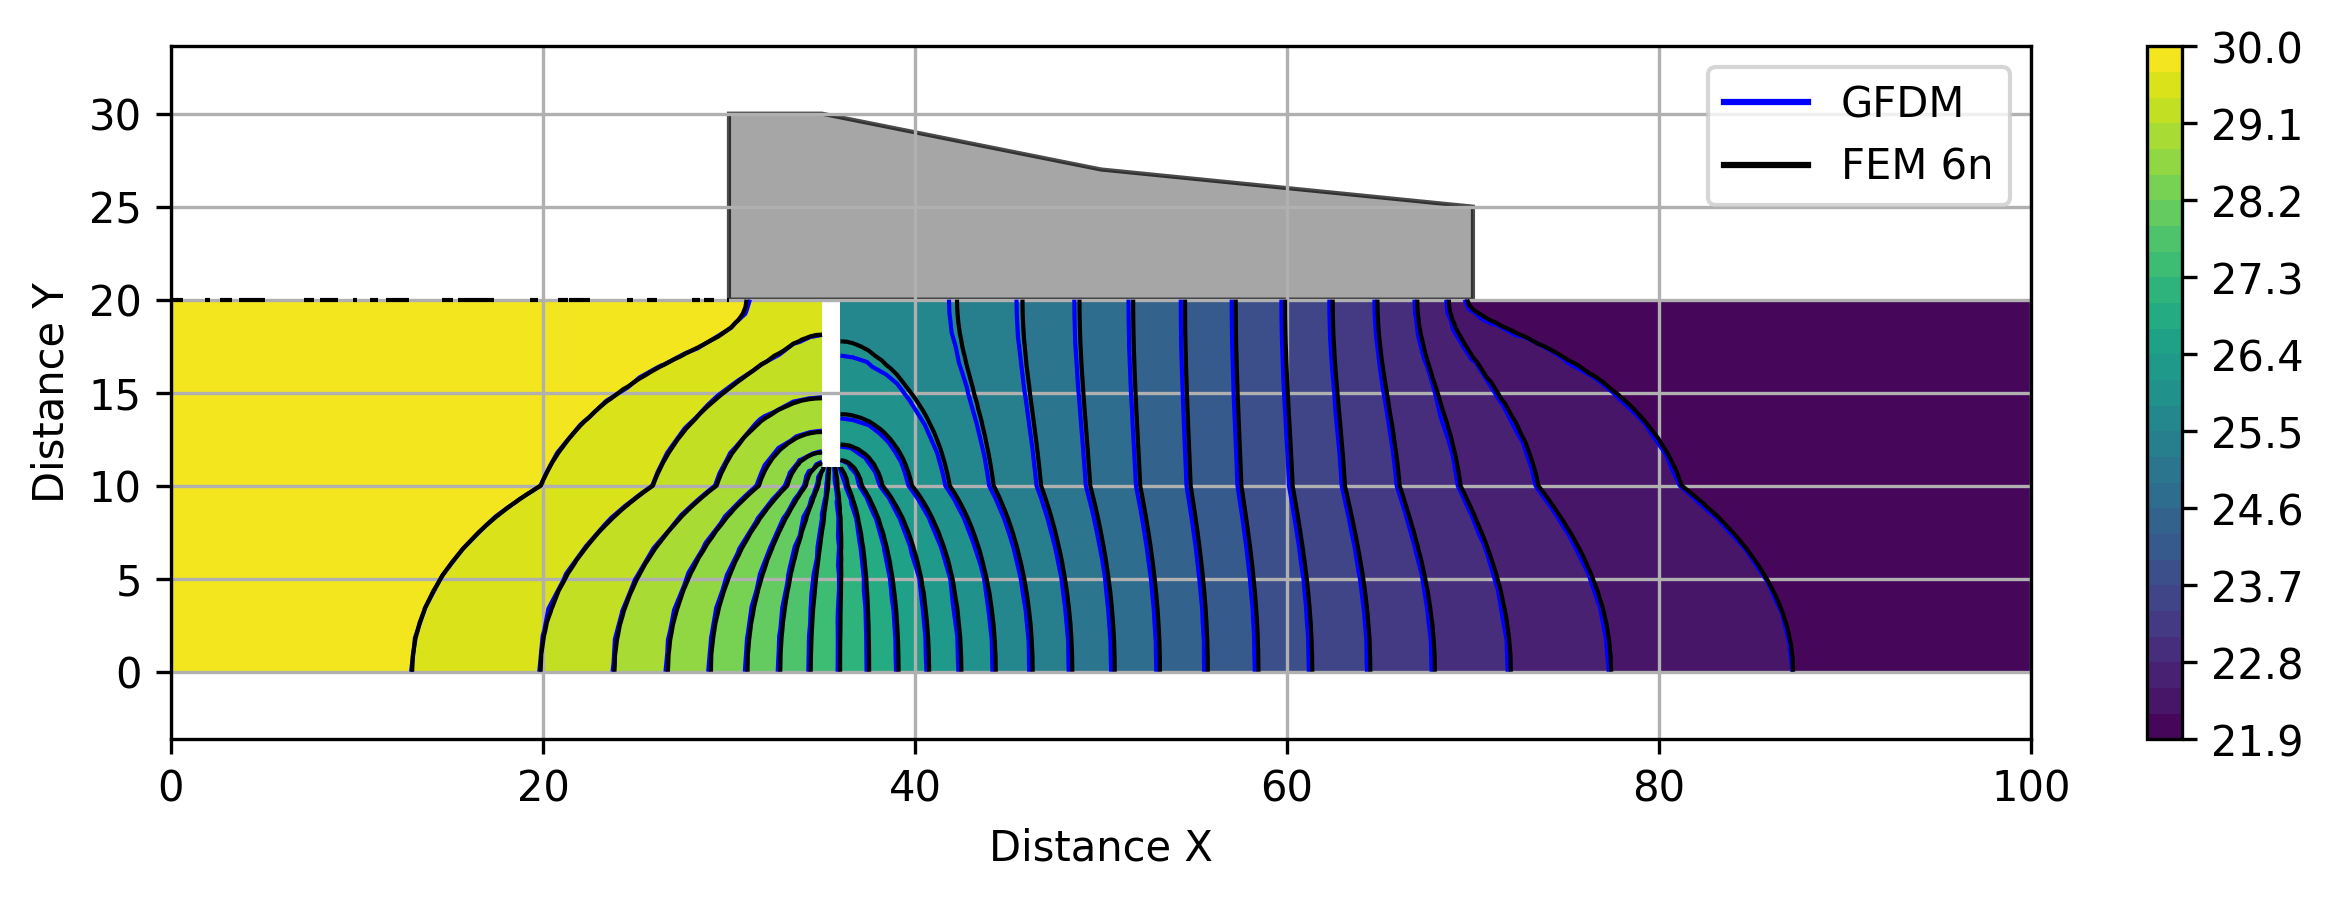
\includegraphics[width=0.9\textwidth]{Presa16nCompara.png}
  \caption{Results for confined seepage in a foundation dam with FEM with 6 nodes elements}
  \label{fig:13}
\end{figure}

\subsubsection{Solution of groundwater flow in two layers of unsaturated Dam}

In this case, the problem has an impervious core that delays the water flow; this is an unsaturated problem. Figure (\ref{fig:14}) shows the domain; 1380 nodes were used to calculate the solution. Figure (\ref{fig:14}) shows the mesh points used. In the figure, the boundary conditions are shown too. On the left-hand side (points in green), the total head value is 8 m. On the right downstream, a filter imposes a water pressure of zero (points in green). The points in red have a normal Neumann boundary condition of zero. The soil parameters are presented in the Table (\ref{table1}). The solution to the problem is shown in Figure (\ref{fig:15}); again, the two contours of the equipotential total head (FEM and GFDM) are displayed. The solutions for the GFDM and FEM methods are similar: the only difference is in the upper zone downstream in a zone of high permeability. The $L_{RMSE}$ norm using both interfaces is 0.0514, while in the entire domain, it is 0.03656.              

\begin{table}[]
\caption{Parameters for two layer dam model}\label{table1}
\begin{tabular*}{\tblwidth}{@{}CCCCC@{}}
\toprule
    Soil & $\theta_{sat}$ & $\alpha (1/kPa)$ & n & $k_{sat}(m/s)$ \\ % Table header row
\midrule
    Rockfill & 0.45 & 1/15 & 1.64 & 1e-05 \\
    Clay core & 0.45 & 1/15 & 1.64 &1e-06\\
\bottomrule
\end{tabular*}
\end{table}

\begin{figure}[htb]
  \centering
  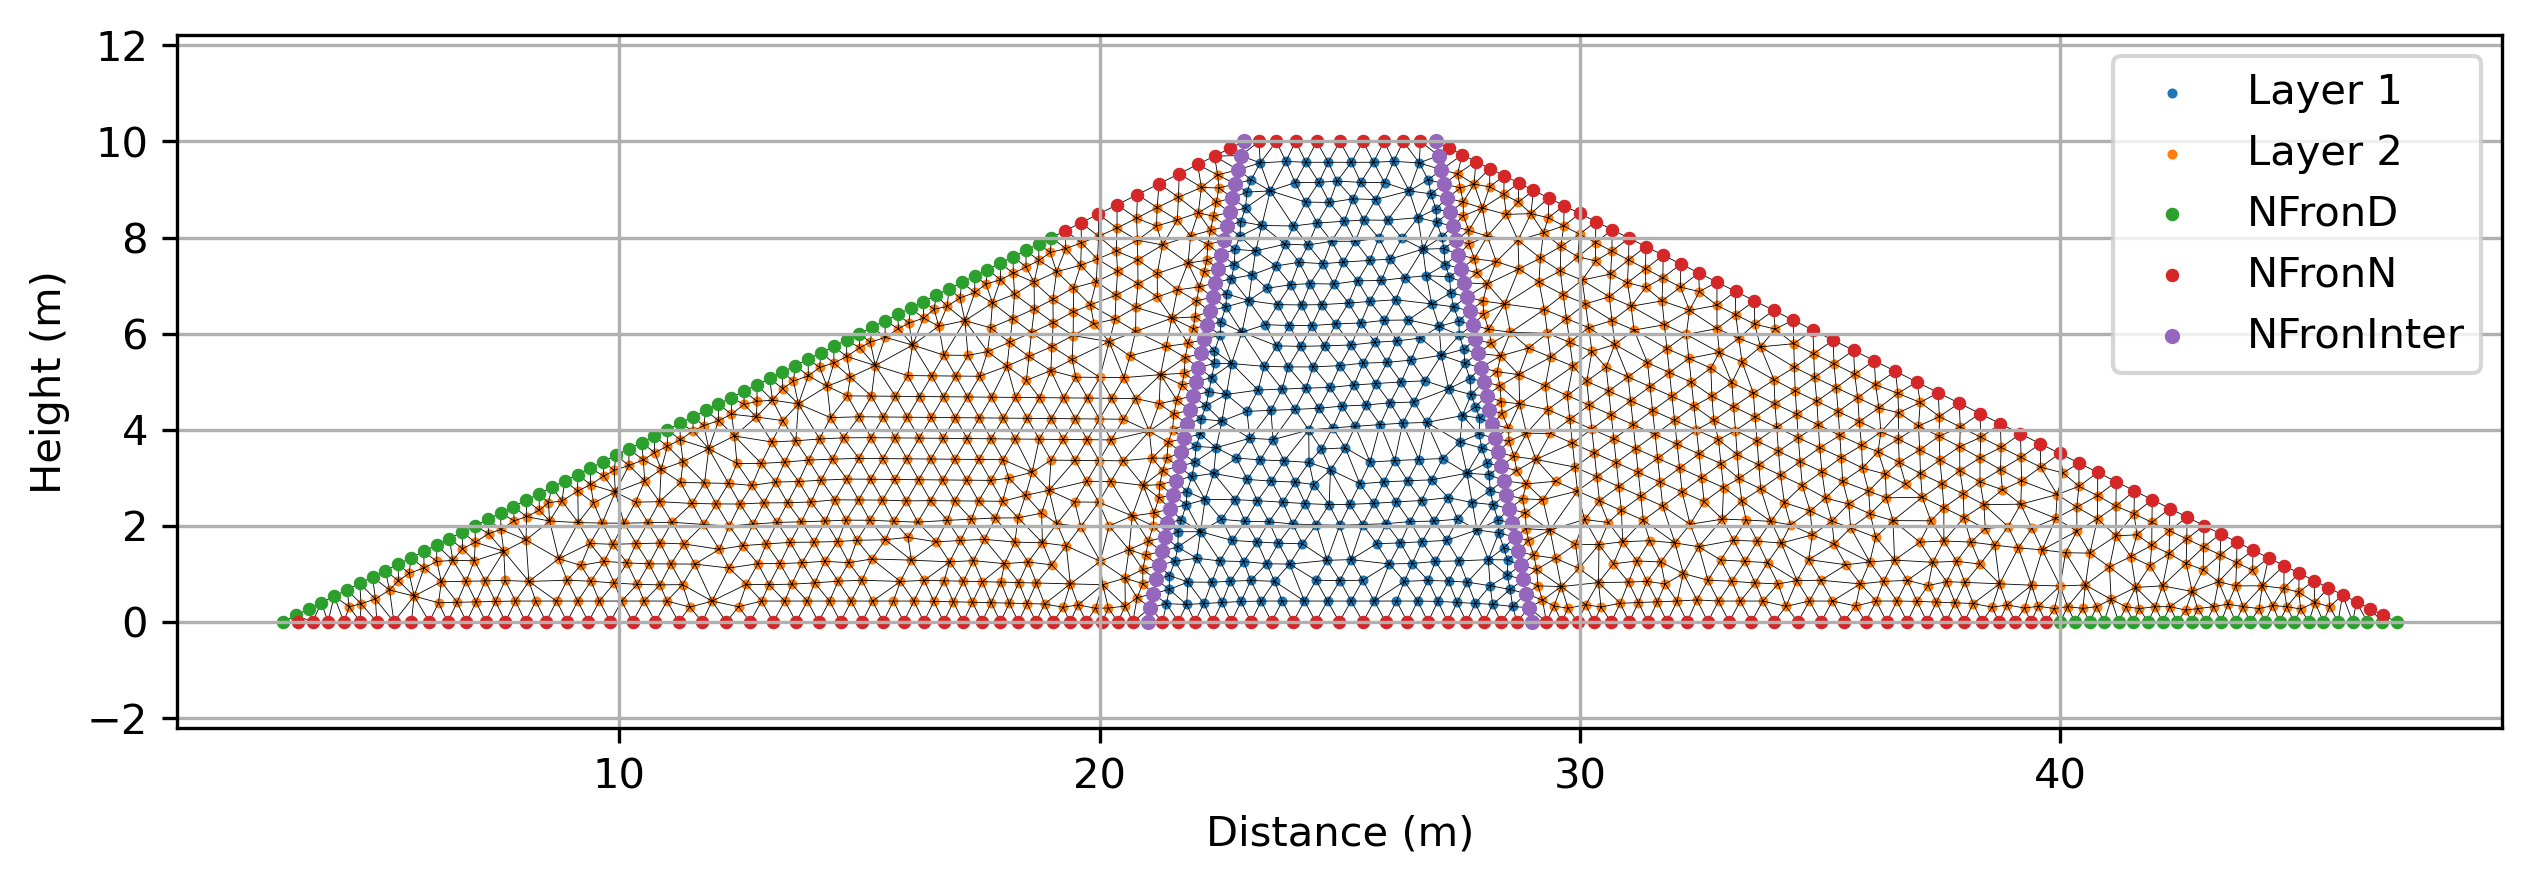
\includegraphics[width=0.9\textwidth]{FigMallaPresa2C.png}
  \caption{Mesh for the two layer dam}
  \label{fig:14}
\end{figure}

\begin{figure}[htb]
  \centering
  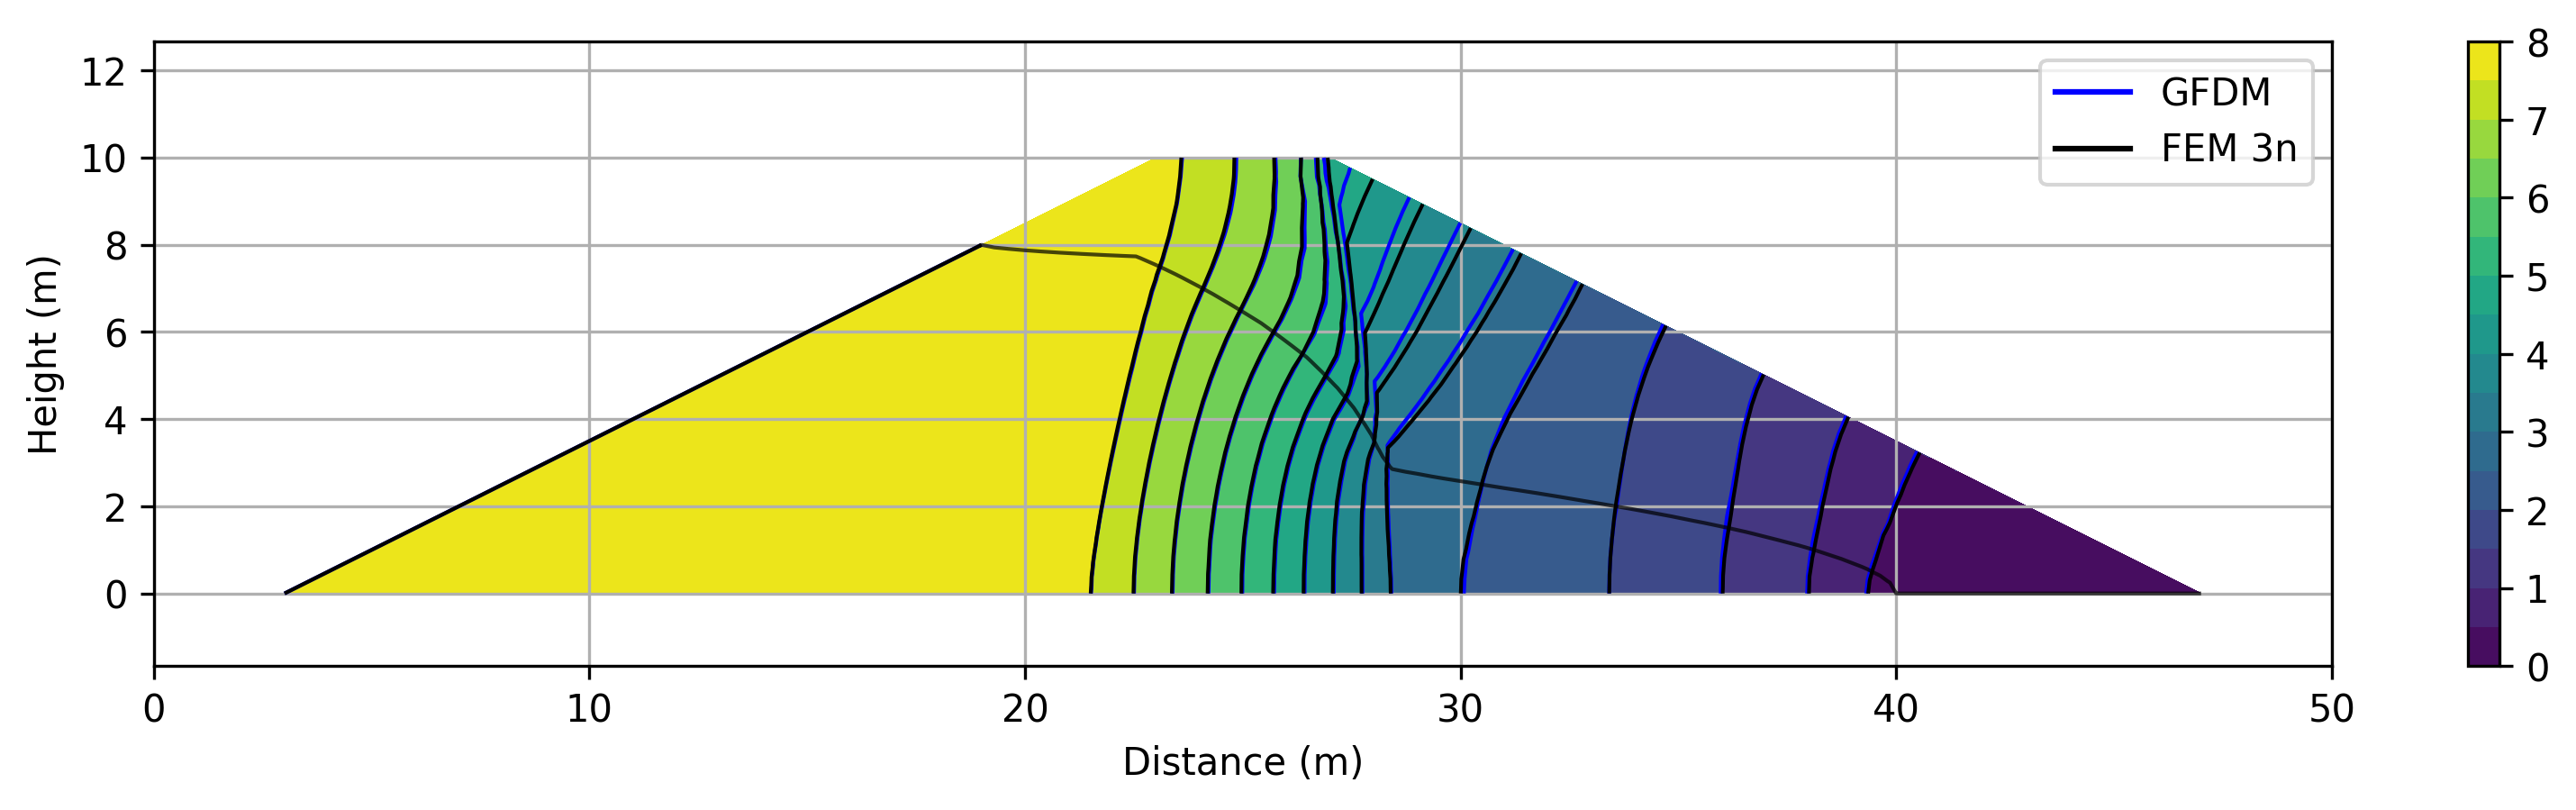
\includegraphics[width=0.9\textwidth]{Presa2Compara.png}
  \caption{total head contours for the two layer dam}
  \label{fig:15}
\end{figure}

\subsubsection{Solution of groundwater flow in five layers Dam}

The case of five layers, tests interfaces with the same properties, and the balance of a point of the three layers are presented in Figure (\ref{fig2}). The dam's geometry is shown in Figure (\ref{fig:16}); there are five layers with three different materials: rockfill, clay core, and soil foundation. The rockfill and the soil foundation have the same properties (see Table \ref{table2}). The red nodes are the Dirichlet boundary conditions; on the left side, the total head equals eight, and on the right side, it equals zero. The domain has a mesh of 1503 nodes; in orange are the nodes of the rockfill, in blue are the nodes of the core, and in green are the nodes of the soil foundation. Figure (\ref{fig:17}) shows the analysis results; both families of equipotential lines are very close. The interface between the rockfill and soil foundation has not changed the solution; there is no visible perturbation in the equipotential lines. The solution on the point of union of the three layers is continuous. The $L_{RMSE}$ norm for the interfaces is 0.107 and 0.114 in general.      

\begin{table}[]
\caption{Parameters for the simulation for five layers problems}\label{table2}
\begin{tabular*}{\tblwidth}{@{}CCCCC@{}}
\toprule
    Soil & $\theta_{sat}$ & $\alpha (1/kPa)$ & n & $k_{sat}(m/s)$ \\% Table header row
\midrule
    Rockfill & 0.5 & 1/50 & 1.4 & 0.0001 \\
    Clay core & 0.5 & 1/50 & 1.4 &1e-06 \\
    Soil Foundation & 0.5 & 1/50 & 1.4 & 0.0001\\
\bottomrule
\end{tabular*}
\end{table}

\begin{figure}[htb]
  \centering
  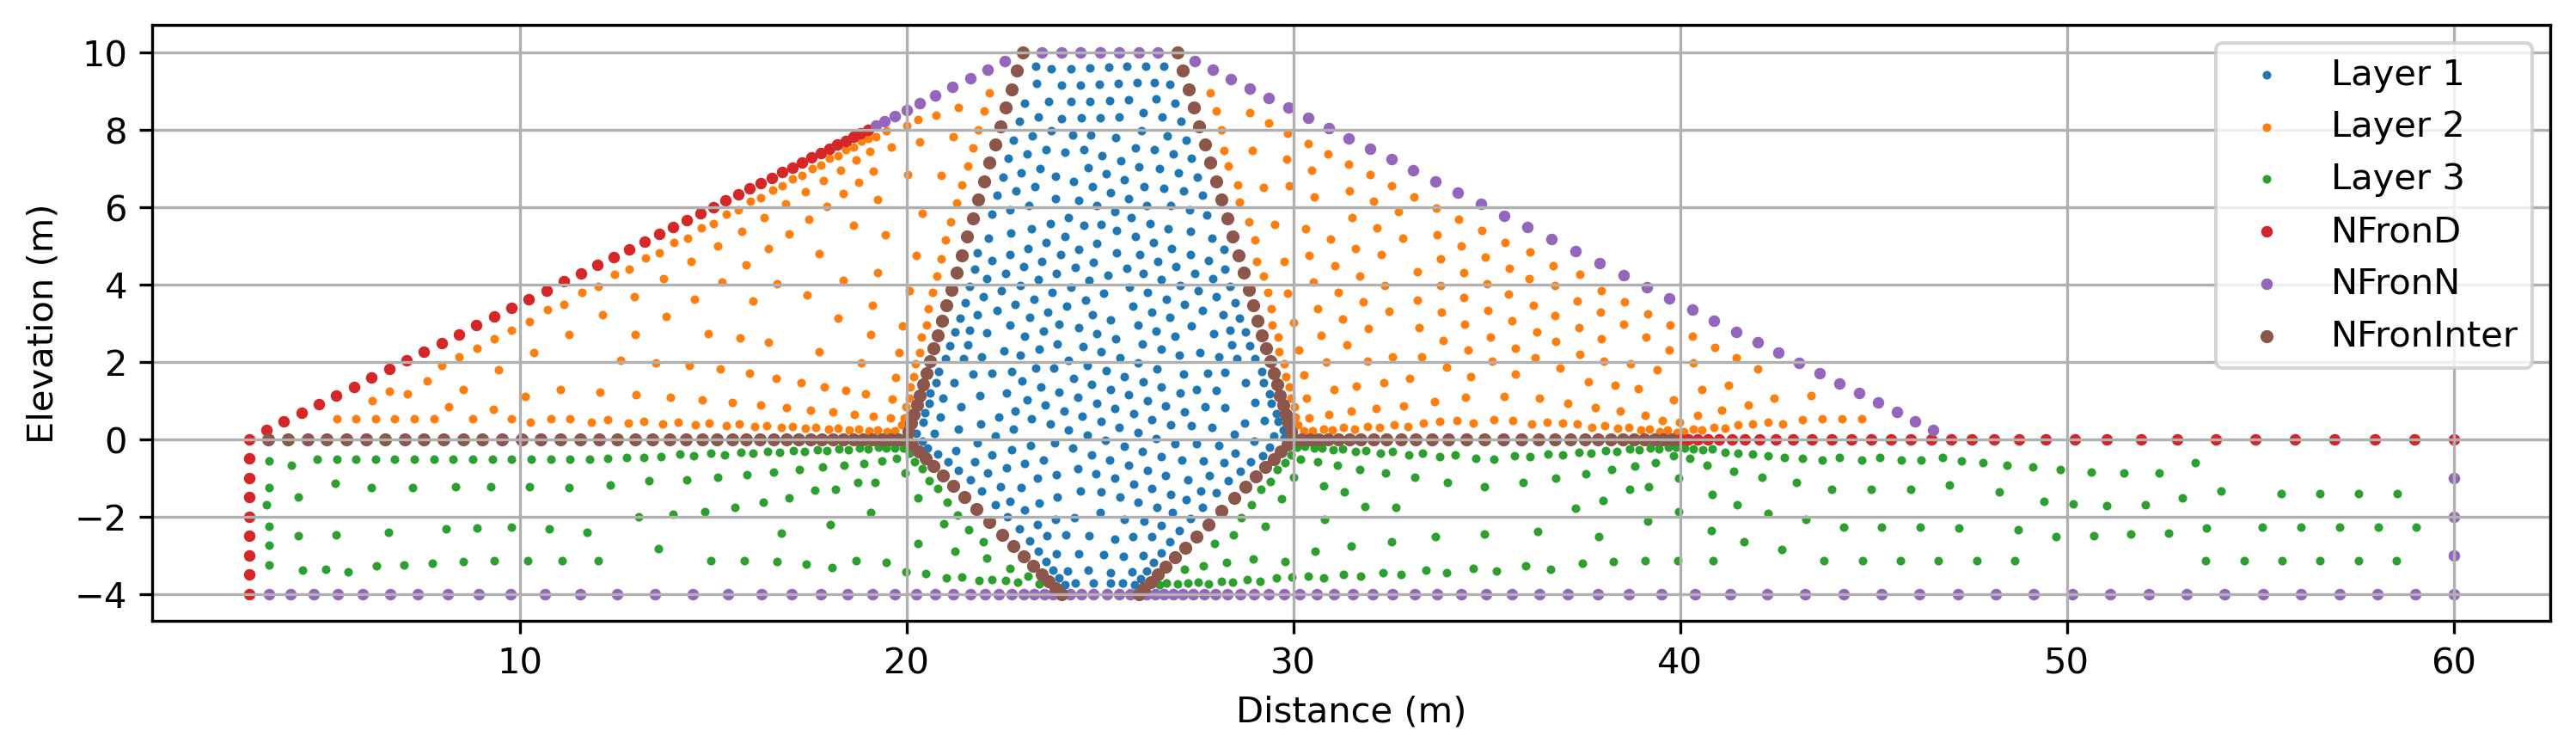
\includegraphics[width=0.9\textwidth]{FigMallaPresa5C.png}
  \caption{Mesh for the analysis of five layer problem}
  \label{fig:16}
\end{figure}

\begin{figure}[htb]
  \centering
  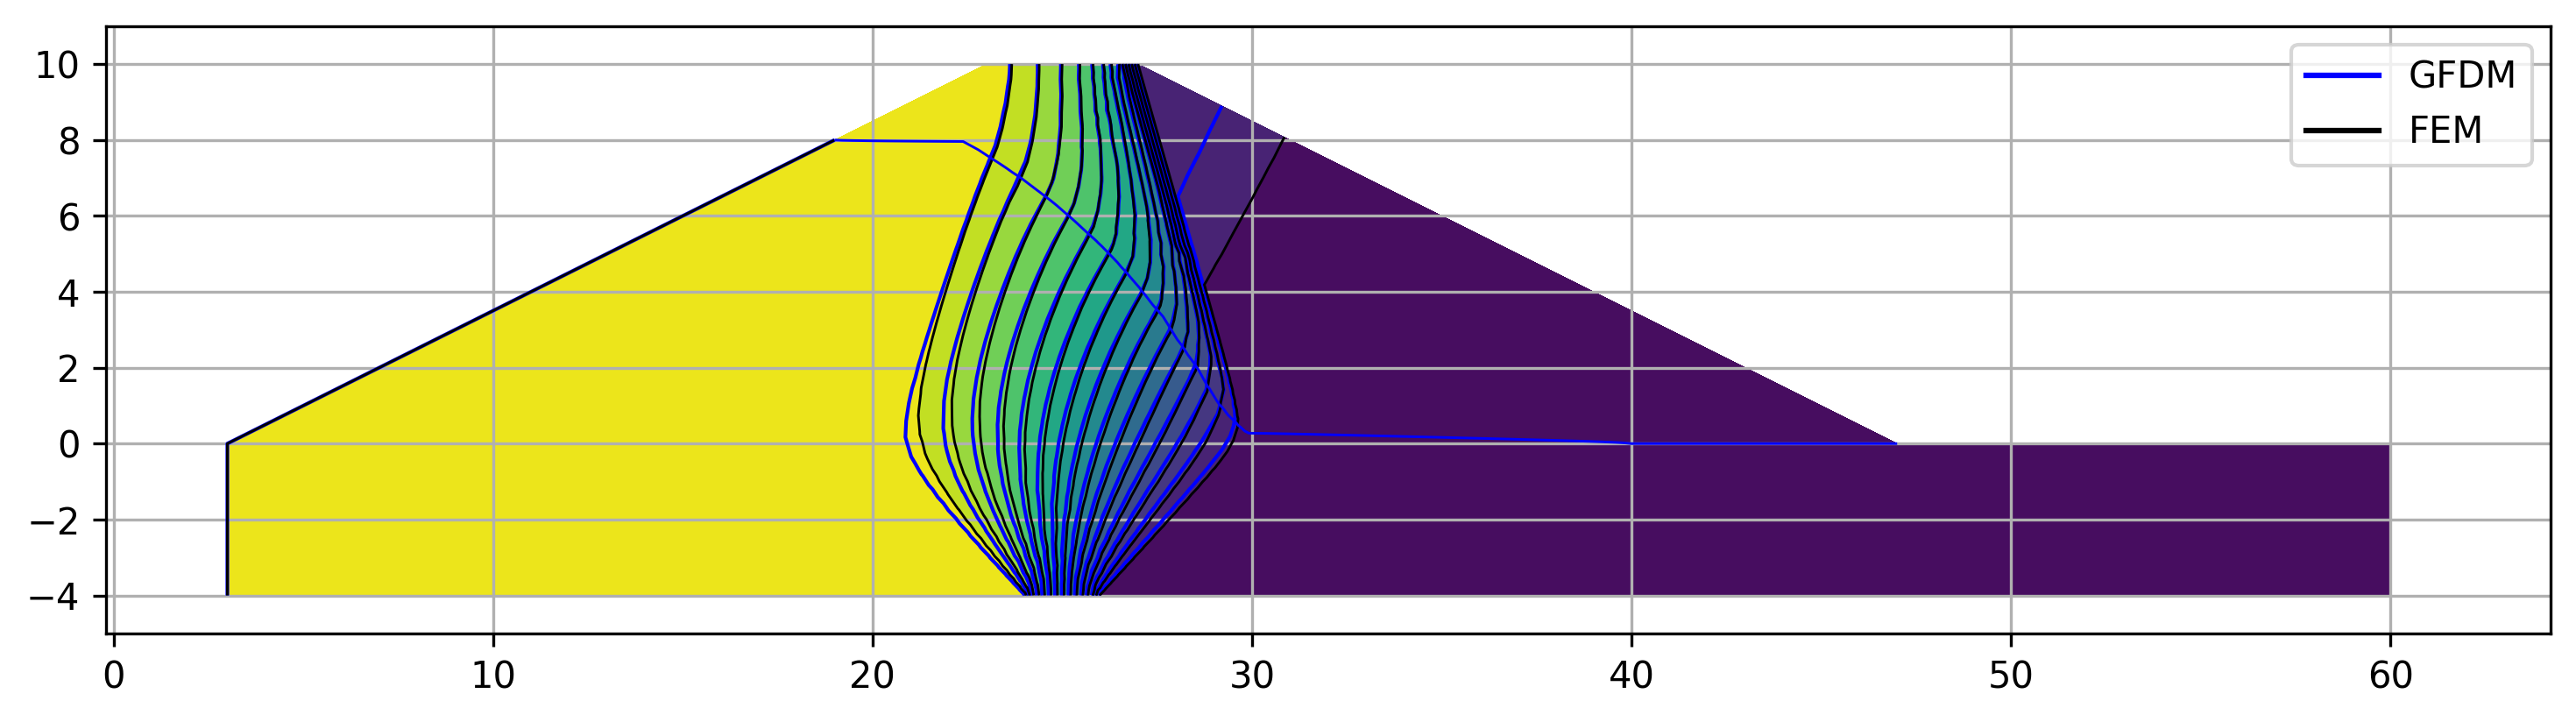
\includegraphics[width=0.96\textwidth]{FigDam5CCompara2.png}
  \caption{Total head contours results of five layer problem}
  \label{fig:17}
\end{figure}

\section{Conclusions}\label{sec5}
A new technique applied to the { unweighted} generalized finite differences method to solve groundwater flow in layered domains was proposed. The approach balances the water flow amount at each interface node. To carry out the balance, the amount of water crossing normal to the interface is calculated, and then the flow balance is made in cartesian components; in the case of stationary flow, the water balance must be equal to zero.

This technique was verified first with three simple interface problems.  The first problem tests the continuity in a vertical interface of a horizontal rectangle with two layers and two coefficients of permeability. To evaluate the results of each test case, a finite element model with the same mesh was solved. In this case, the GFDM and FEM produce the same results, with a norm $L_{RMSE}$ in the interface of 3.473-14. The second problem tests the inclined interface of two materials. In this case, a slight displacement in equipotential lines in the zone of the material with less permeability can be noticed; the norm $L_{RMSE}$ obtained in the interface nodes was 0.094. The third case tests the point of the interface with three materials in a square domain. The solution matched better than the previous example; there is a slight displacement in the equipotential lines in the zone of less permeability; this produces a $L_{RSME}$ norm of 0.042 in the interface. If we analyze the mesh for the two last problems, we can observe the better quality of the mesh of the third problem. As expected, if the mesh is more refined, the difference between the GFDM and FEM calculated values is lower. {From Equation (\ref{eq6}), it can be seen that is also possible to increase $q$, the number of support nodes, to increase accuracy and order in the approximation. This suggests that a finer mesh can be used to produce more accurate results. However, acceptable values were obtained using a rather low number of nodes. Bearing in mind the simplicity of the formulation, this is a remarkable feature of the GFDM.}

The solution of groundwater flow in geotechnical problems tests other capabilities of the method, such as the more complex boundary in the case of the confined seepage, the solution to the nonlinear problems (the last two dams), and the continuity of the solution between two zones of a problem with the same properties (dam of five layers). An interesting finding was that modeling the groundwater flow of a confined seepage foundation with a mesh with more elements with FEM perfectly matches the solution of GFDM presented with the original mesh (Figure \ref{fig:13}). It means that GFDM, in this test, shows slightly more accurate results than the FEM, {even though these layered problems are characterized by discontinuous coefficients.} In the case of the two-layer dam, the tendency of the solution is very similar in both methods. The most significant deviations occur in the areas with the lowest permeability.  

As final reflections, it's worth noting that since both methods are based on different discretization procedures using different local polynomials, this explains the variation in nodal values. However, these values tend to converge and get closer in a refined mesh, as expected. It can also be said that the proposed balance in the interface nodes leads to a good approximation, and this reveals certain advantages of GFDM over FEM. Despite the presence of discontinuities, which can be managed with generalized differences, the proposed methodology for modeling layered domain problems is suitable for delivering accurate approximations.

% Numbered list
% Use the style of numbering in square brackets.
% If nothing is used, default style will be taken.
%\begin{enumerate}[a)]
%\item 
%\item 
%\item 
%\end{enumerate}  

% Unnumbered list
%\begin{itemize}
%\item 
%\item 
%\item 
%\end{itemize}  

% Description list
%\begin{description}
%\item[]
%\item[] 
%\item[] 
%\end{description}  

%%%% Figure
%%%\begin{figure}[<options>]
%%%	\centering
%%%		\includegraphics[<options>]{}
%%%	  \caption{}\label{fig1}
%%%\end{figure}


%%%\begin{table}[<options>]
%%%\caption{}\label{tbl1}
%%%\begin{tabular*}{\tblwidth}{@{}LL@{}}
%%%\toprule
%%%  &  \\ % Table header row
%%%\midrule
%%% & \\
%%% & \\
%%% & \\
%%% & \\
%%%\bottomrule
%%%\end{tabular*}
%%%\end{table}

% Uncomment and use as the case may be
%\begin{theorem} 
%\end{theorem}

% Uncomment and use as the case may be
%\begin{lemma} 
%\end{lemma}

%% The Appendices part is started with the command \appendix;
%% appendix sections are then done as normal sections
%% \appendix

% To print the credit authorship contribution details
\printcredits

%% Loading bibliography style file
%\bibliographystyle{model1-num-names}
\bibliographystyle{cas-model2-names}

% Loading bibliography database
\bibliography{DosMediosBib.bib}

% Biography
%\bio{{\bf Carlos Chávez-Negrete} is a professor of in the Civil Engineering School of the Universidad Michoa- cana de San Nicolás de Hidalgo (UMSNH) in Morelia, Mexico. He holds a Ph.D. in Geotechnical Engineering from Universitat Politècnica de Catalunya, in Spain. His research interest includes laboratory characterization of soils and rocks, slope stability analysis, pavement analysis, and design, the development of numerical methods for geotechnical engineering, and unsaturated soil mechanics.}
%% Here goes the biography details.
%\endbio
%
%\bio{pic1}
%% Here goes the biography details.
%\endbio
%
%\bio{{\bf Francisco Domínguez-Mota} completed a B.Sc. in Physics and Mathematics at the Universidad Michoacana in México. He obtained a Master degree in Applied Mathematics from the Center of Research in Mathematics in Guanajuato, Mexico, and a Ph.D in Mathematics at the Universidad Nacional Autónoma de México. He is a member of the National System of Researchers (SNI) in México, and is a researcher in Applied Mathematics at the Universidad Michoacana. His areas of research include numerical solution of differential equations and applications in engineering, numerical generation of structured grids and applications of optimization in large scale problems.}
%% Here goes the biography details.
%\endbio
%
%\bio{pic2}
%% Here goes the biography details.
%\endbio
%
%\bio{{\bf Ricardo Rom\'an Guti\'errez} always smiles.}
%% Here goes the biography details.
%\endbio
%
%\bio{pic3}
%% Here goes the biography details.
%\endbio
\end{document}

